\chapter{Fits}

\section{\unit{36}{\invpb}}

\begin{figure}
  \begin{center}
% bottom right top left
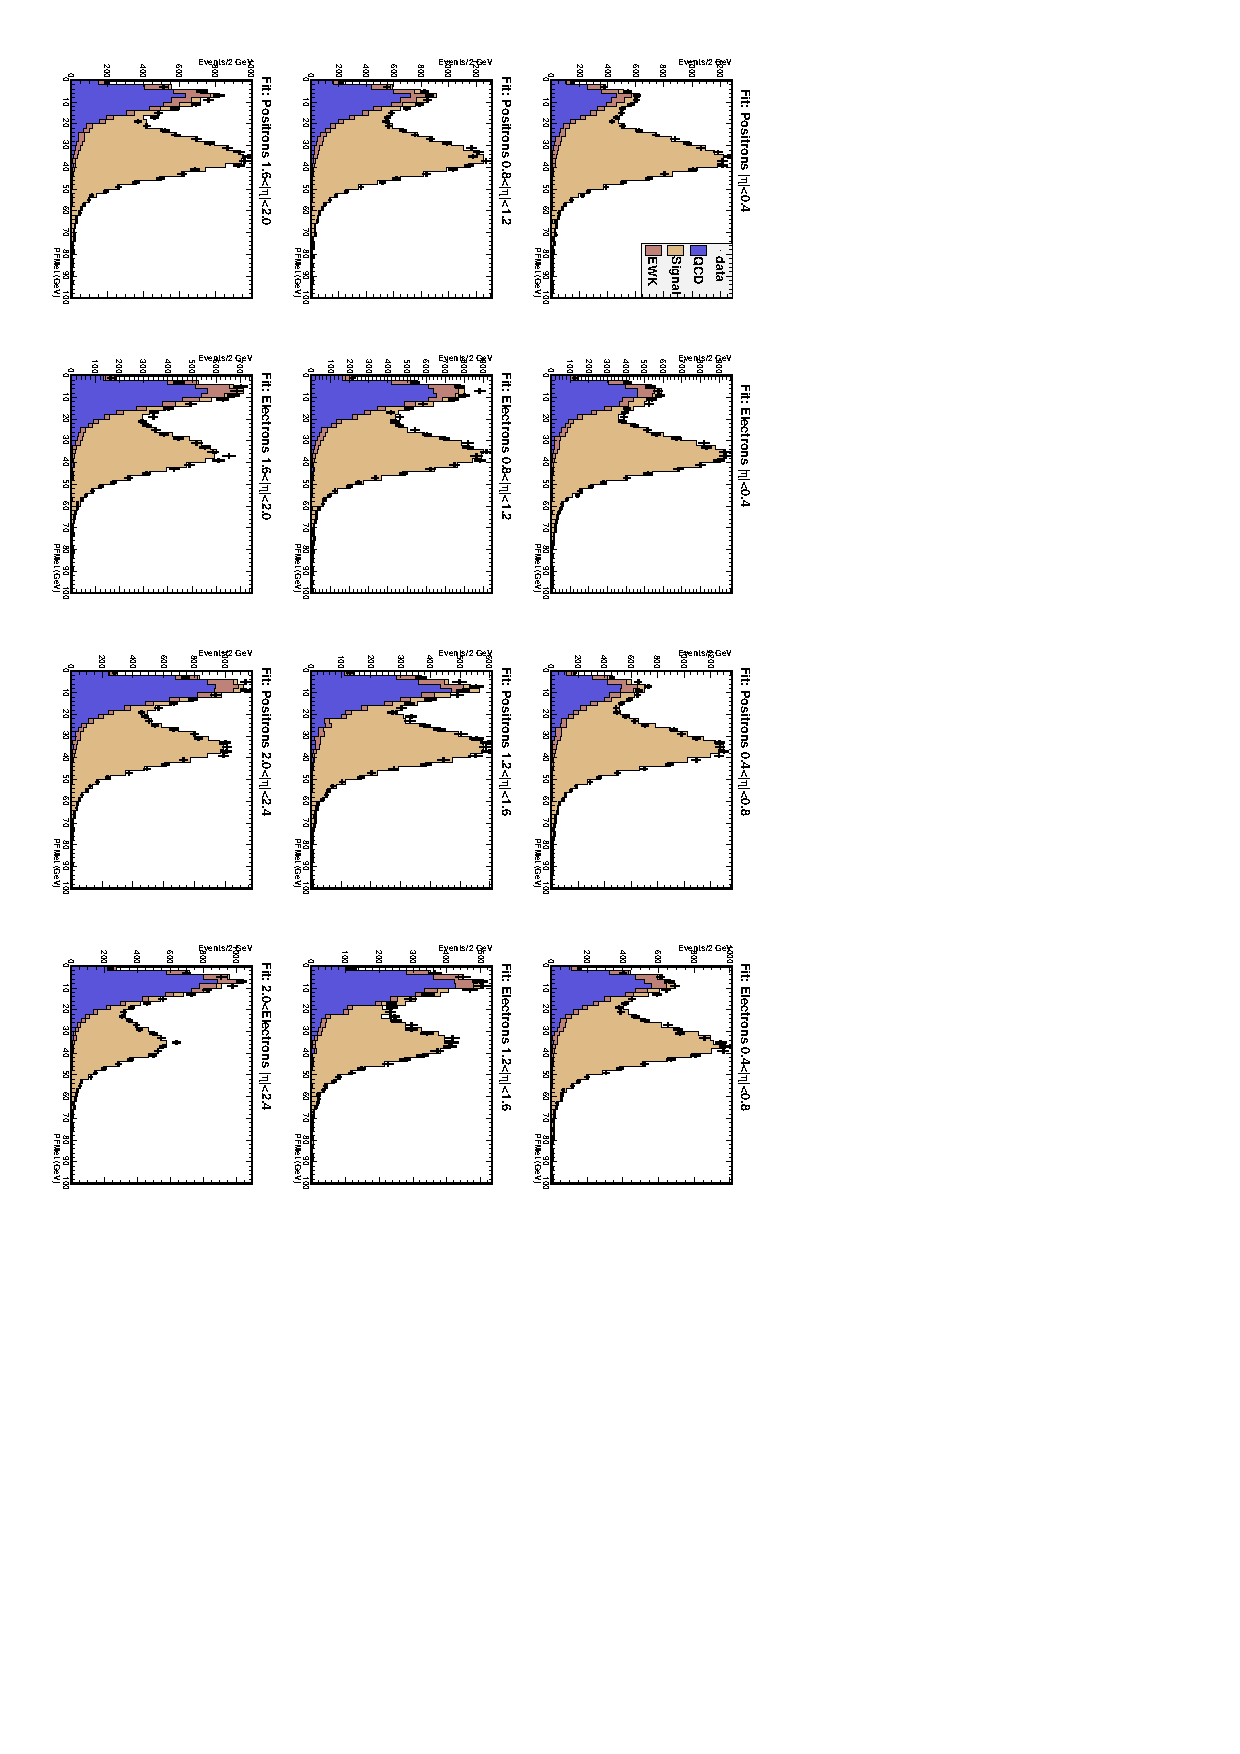
\includegraphics[trim = 80mm 100mm 0mm 0mm, clip, angle=90, width=0.95\textwidth]{Dec22_data}
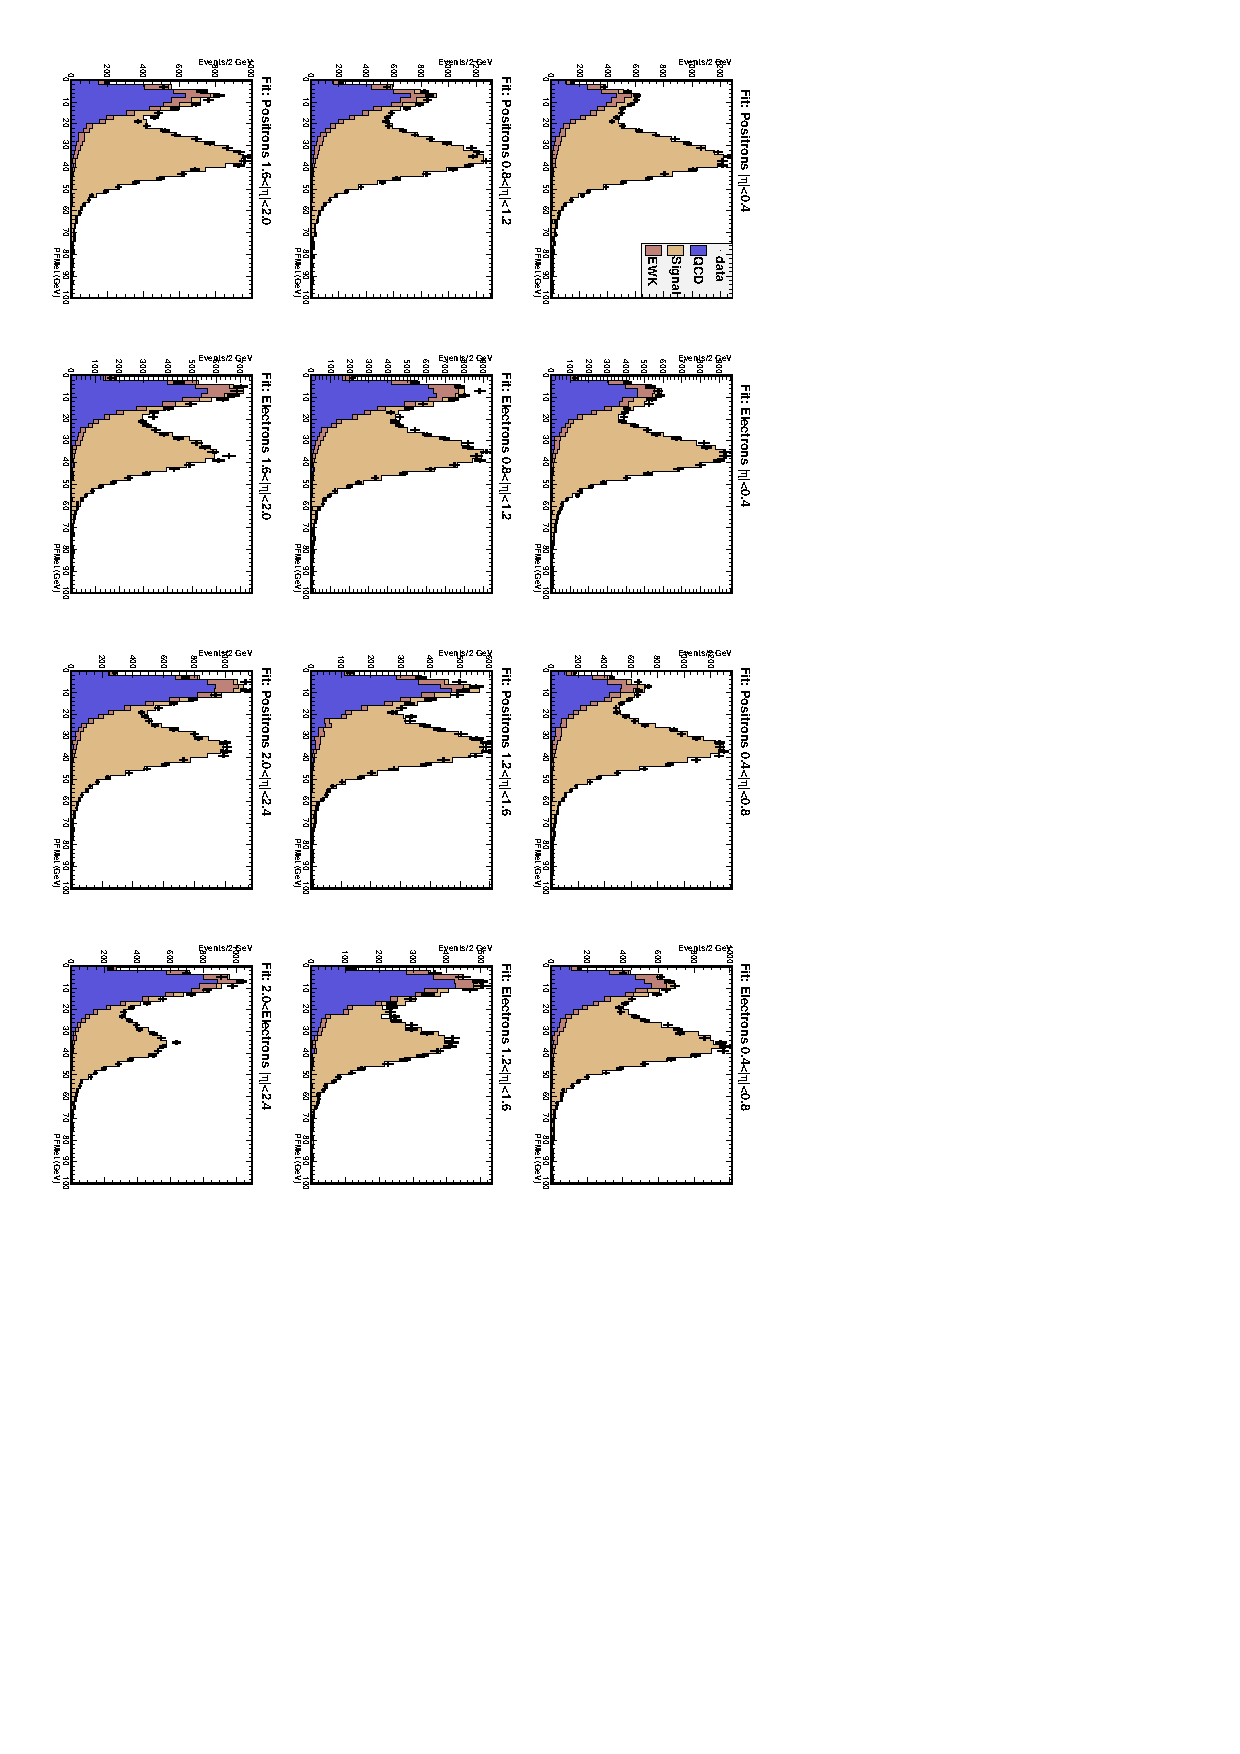
\includegraphics[trim = 80mm 0mm 0mm 100mm, clip, angle=90, width=0.95\textwidth]{Dec22_data}
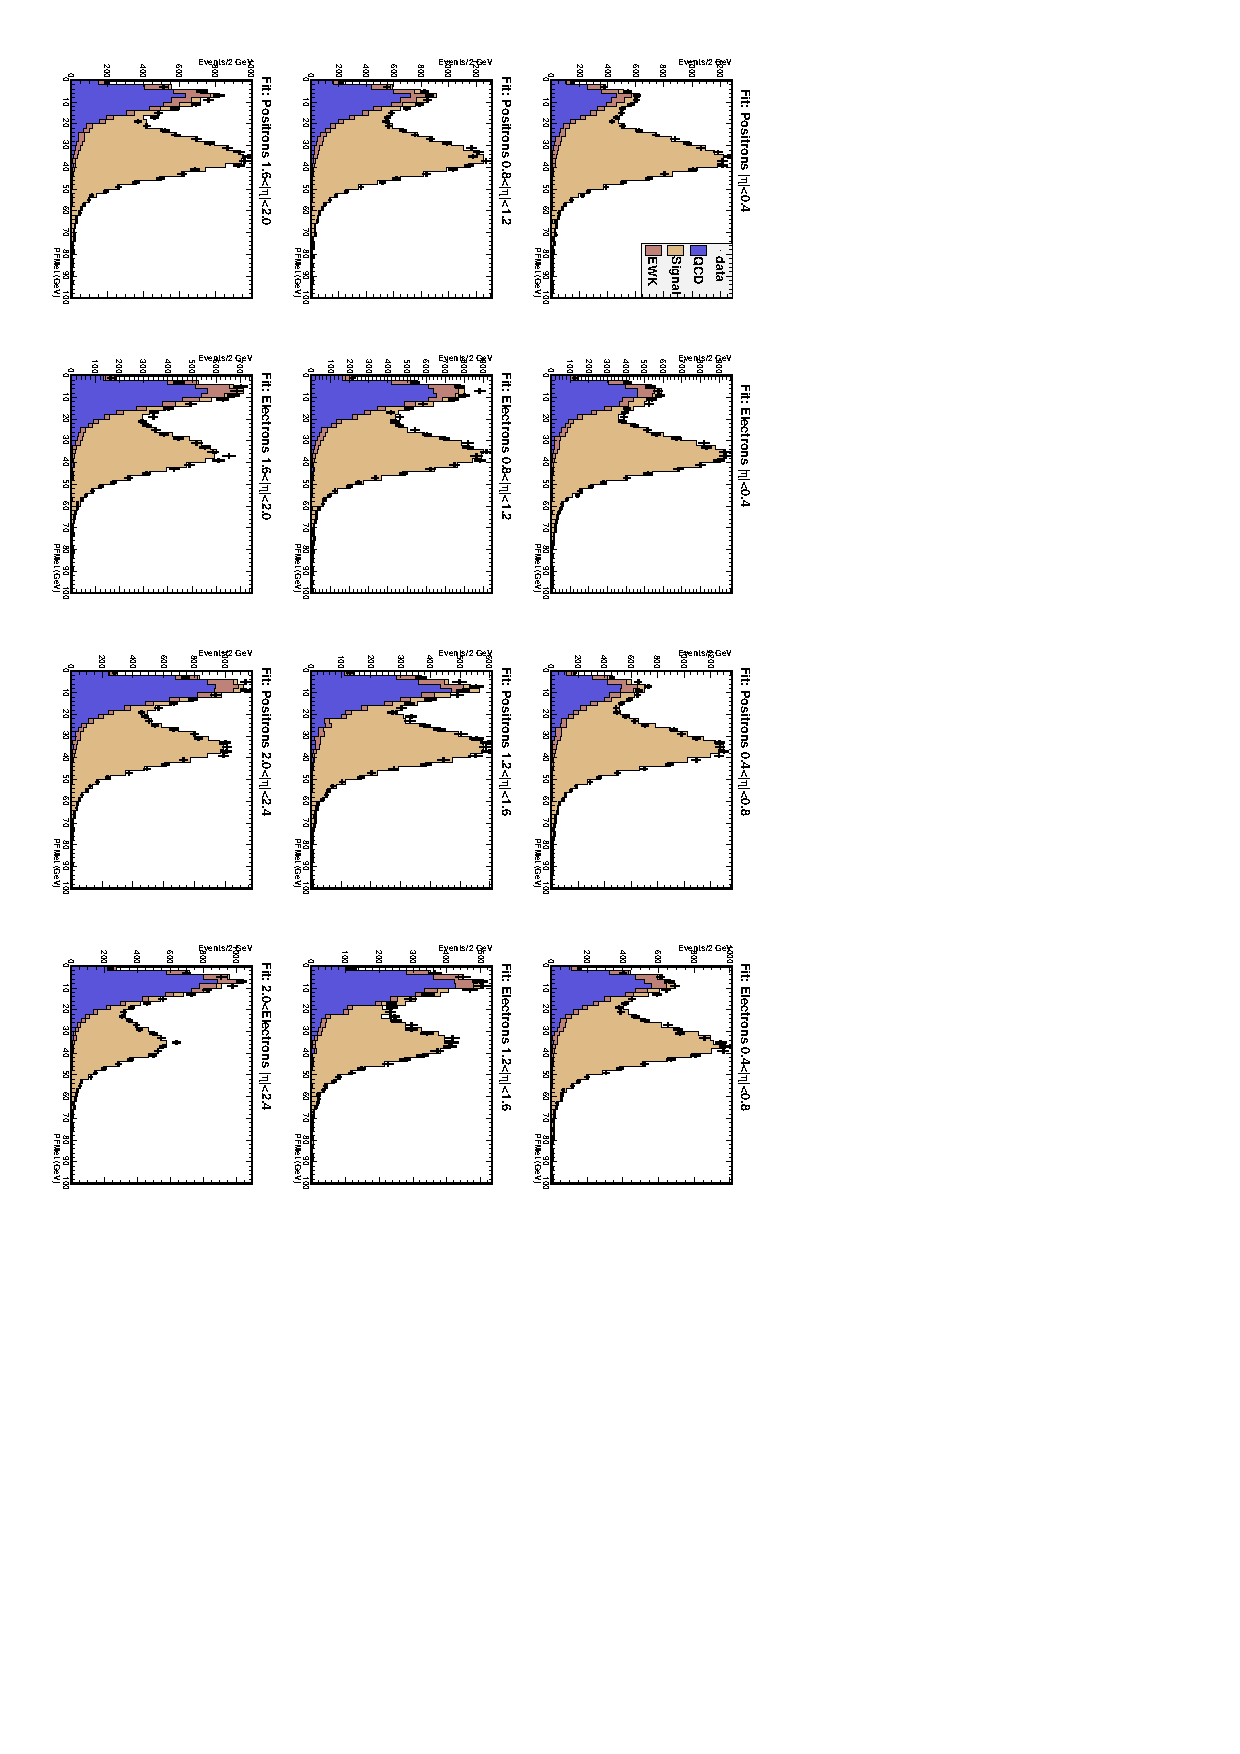
\includegraphics[trim = 40mm 100mm 40mm 0mm, clip, angle=90, width=0.95\textwidth]{Dec22_data}
 \caption{  \label{fig:fit1} The fit to \ETm\ for each eta/charge bin.}
  \end{center}
\end{figure}

\begin{figure}
  \begin{center}
% bottom right top left
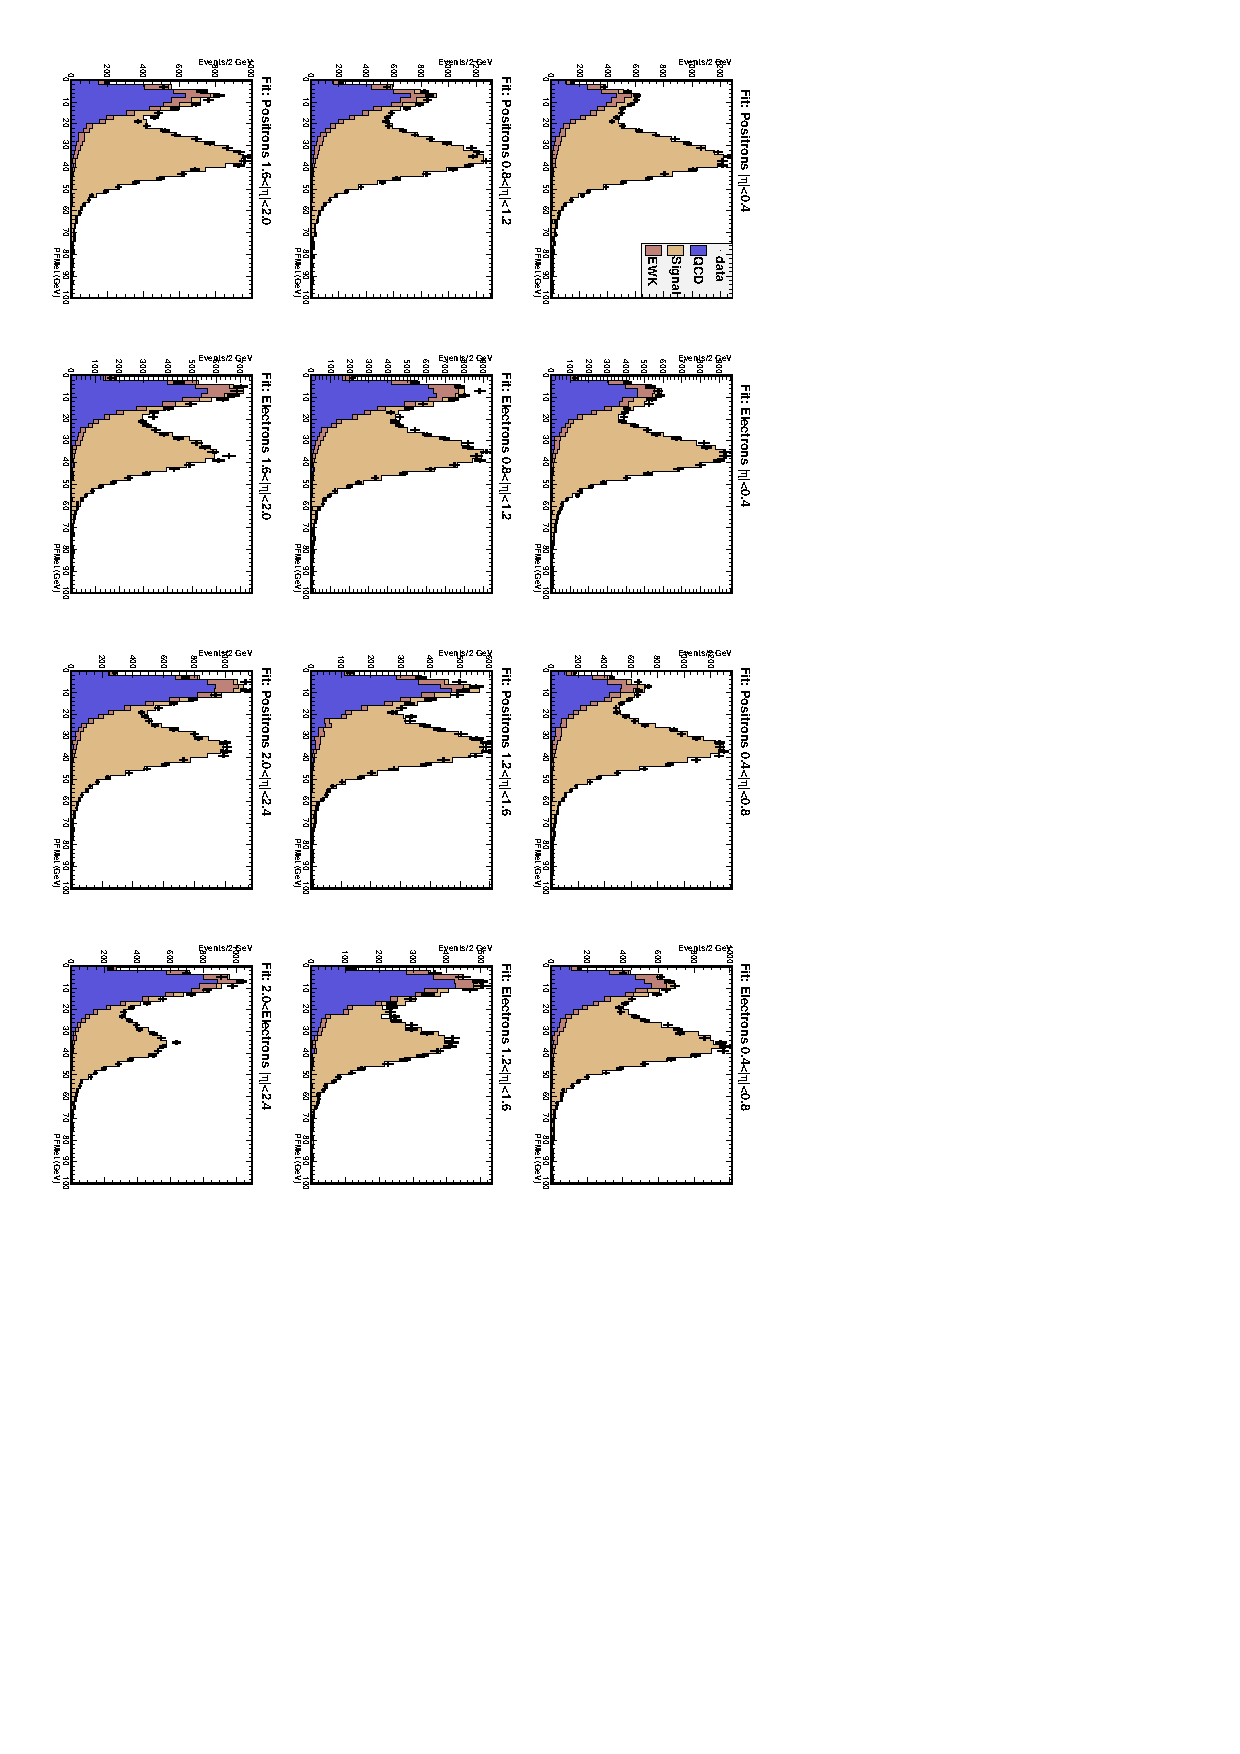
\includegraphics[trim = 40mm 0mm 40mm 100mm, clip, angle=90, width=0.95\textwidth]{Dec22_data}
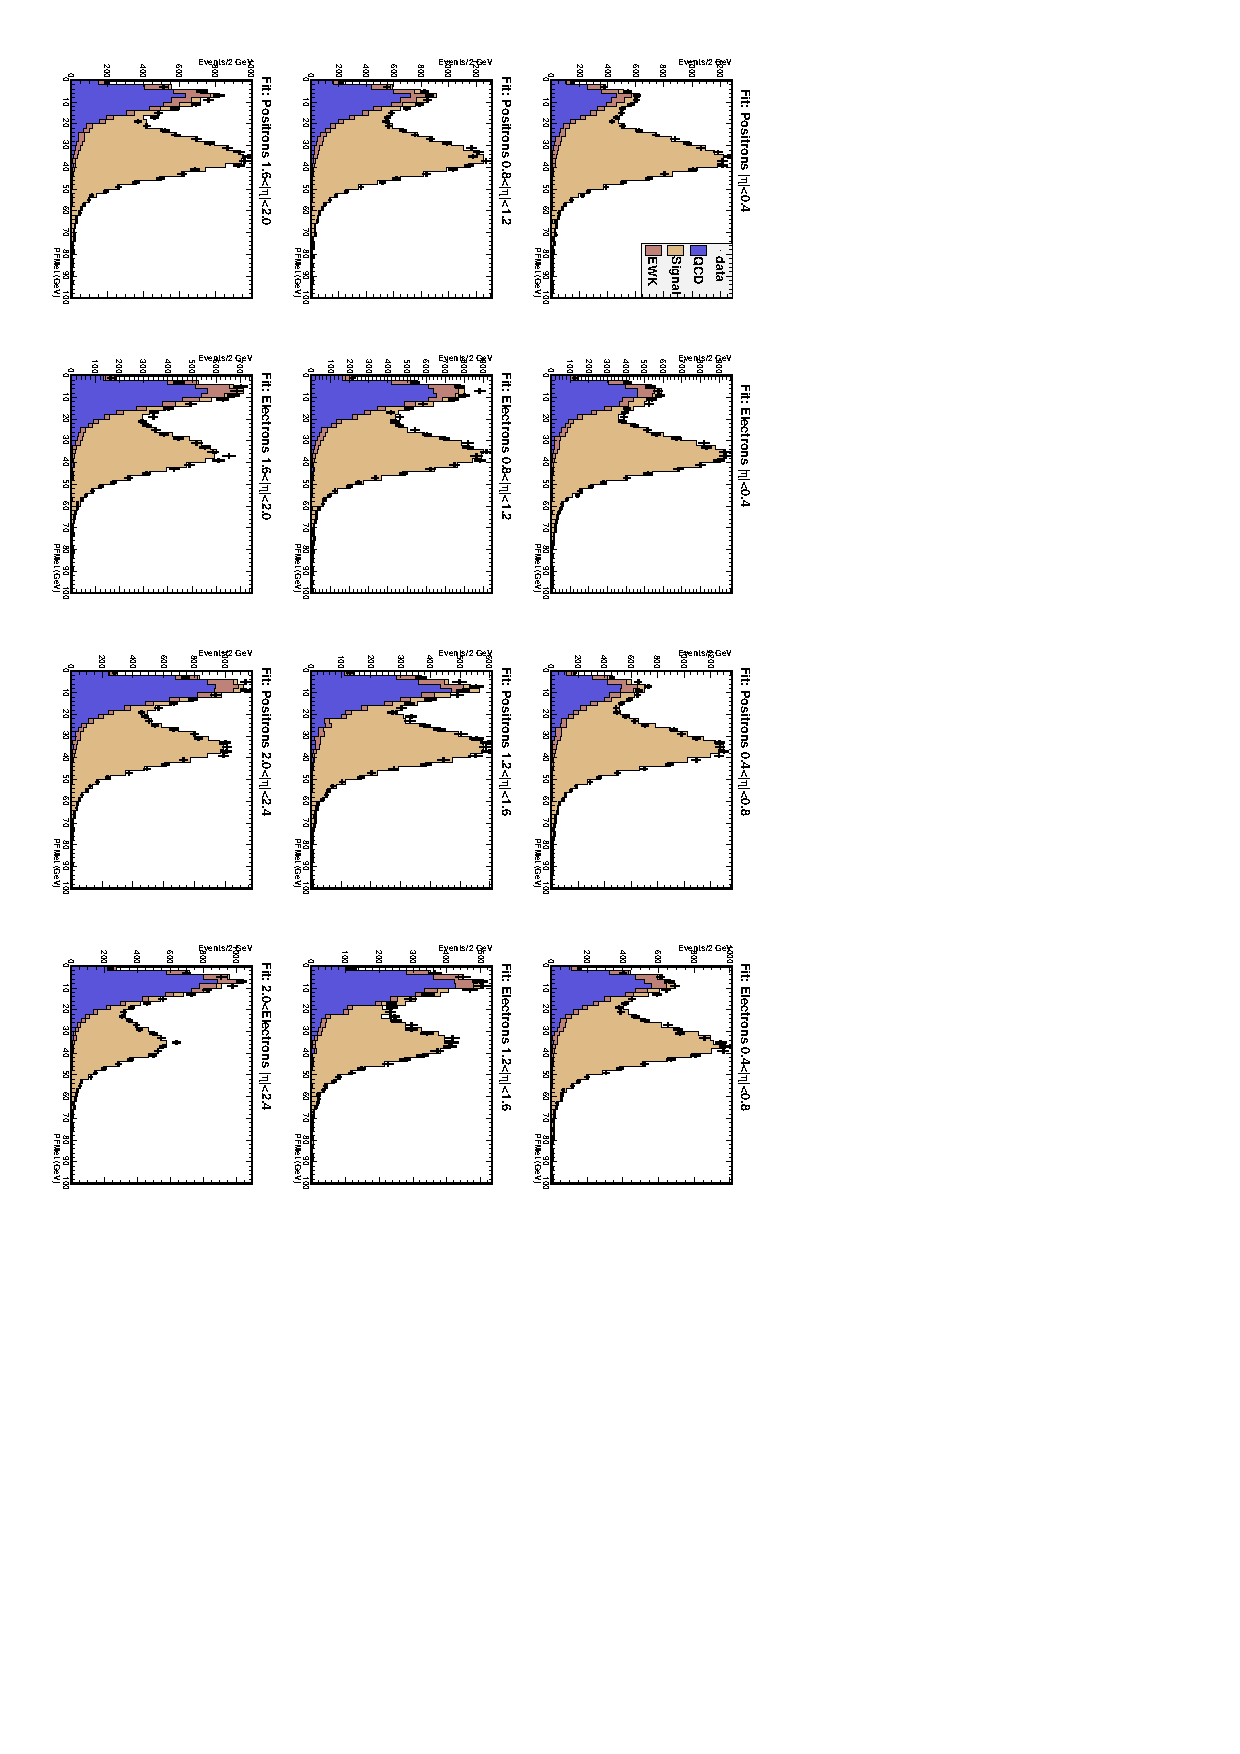
\includegraphics[trim = 0mm 100mm 80mm 0mm, clip, angle=90, width=0.95\textwidth]{Dec22_data}
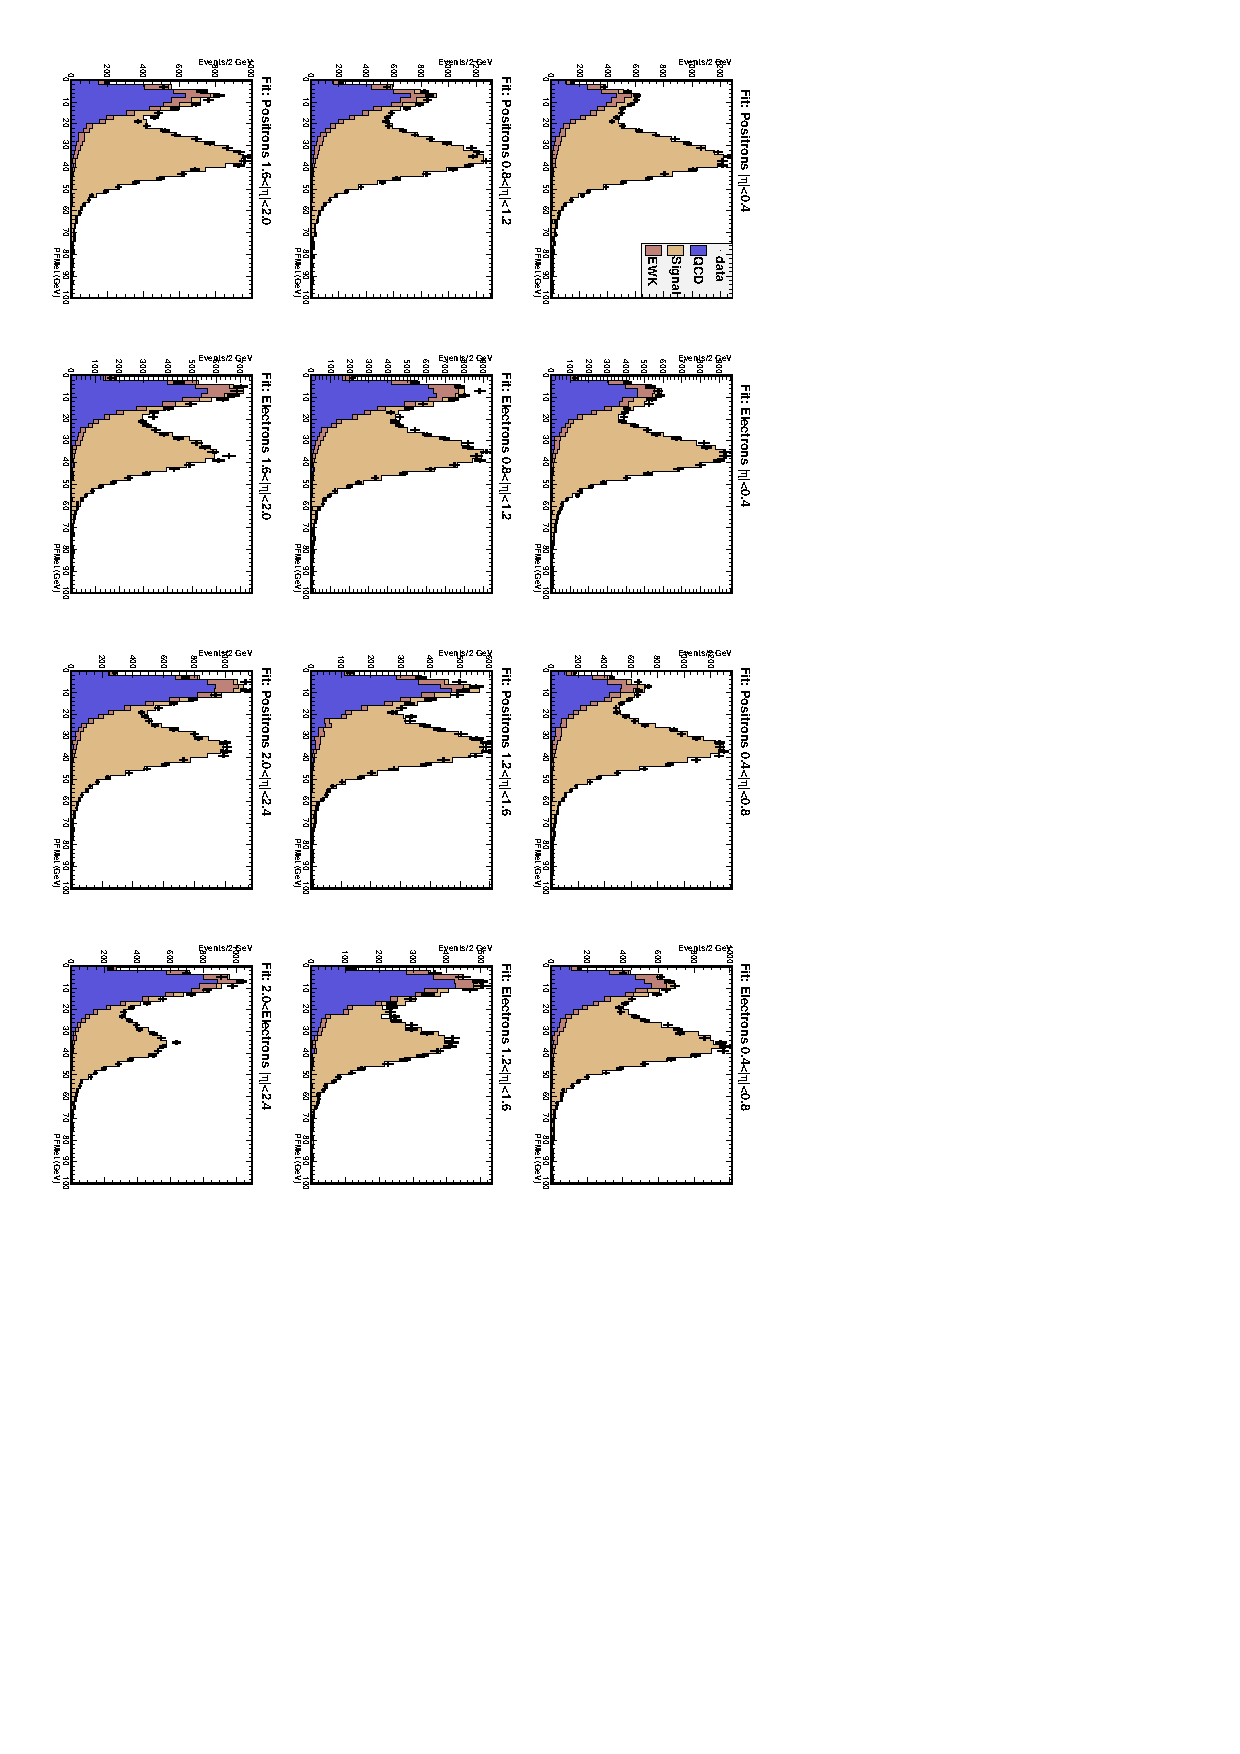
\includegraphics[trim = 0mm 0mm 80mm 100mm, clip, angle=90, width=0.95\textwidth]{Dec22_data}
 \caption{  \label{fig:fit2} The fit to \ETm\ for each eta/charge bin.}
  \end{center}
\end{figure}

\begin{figure}
  \begin{center}
% bottom right top left
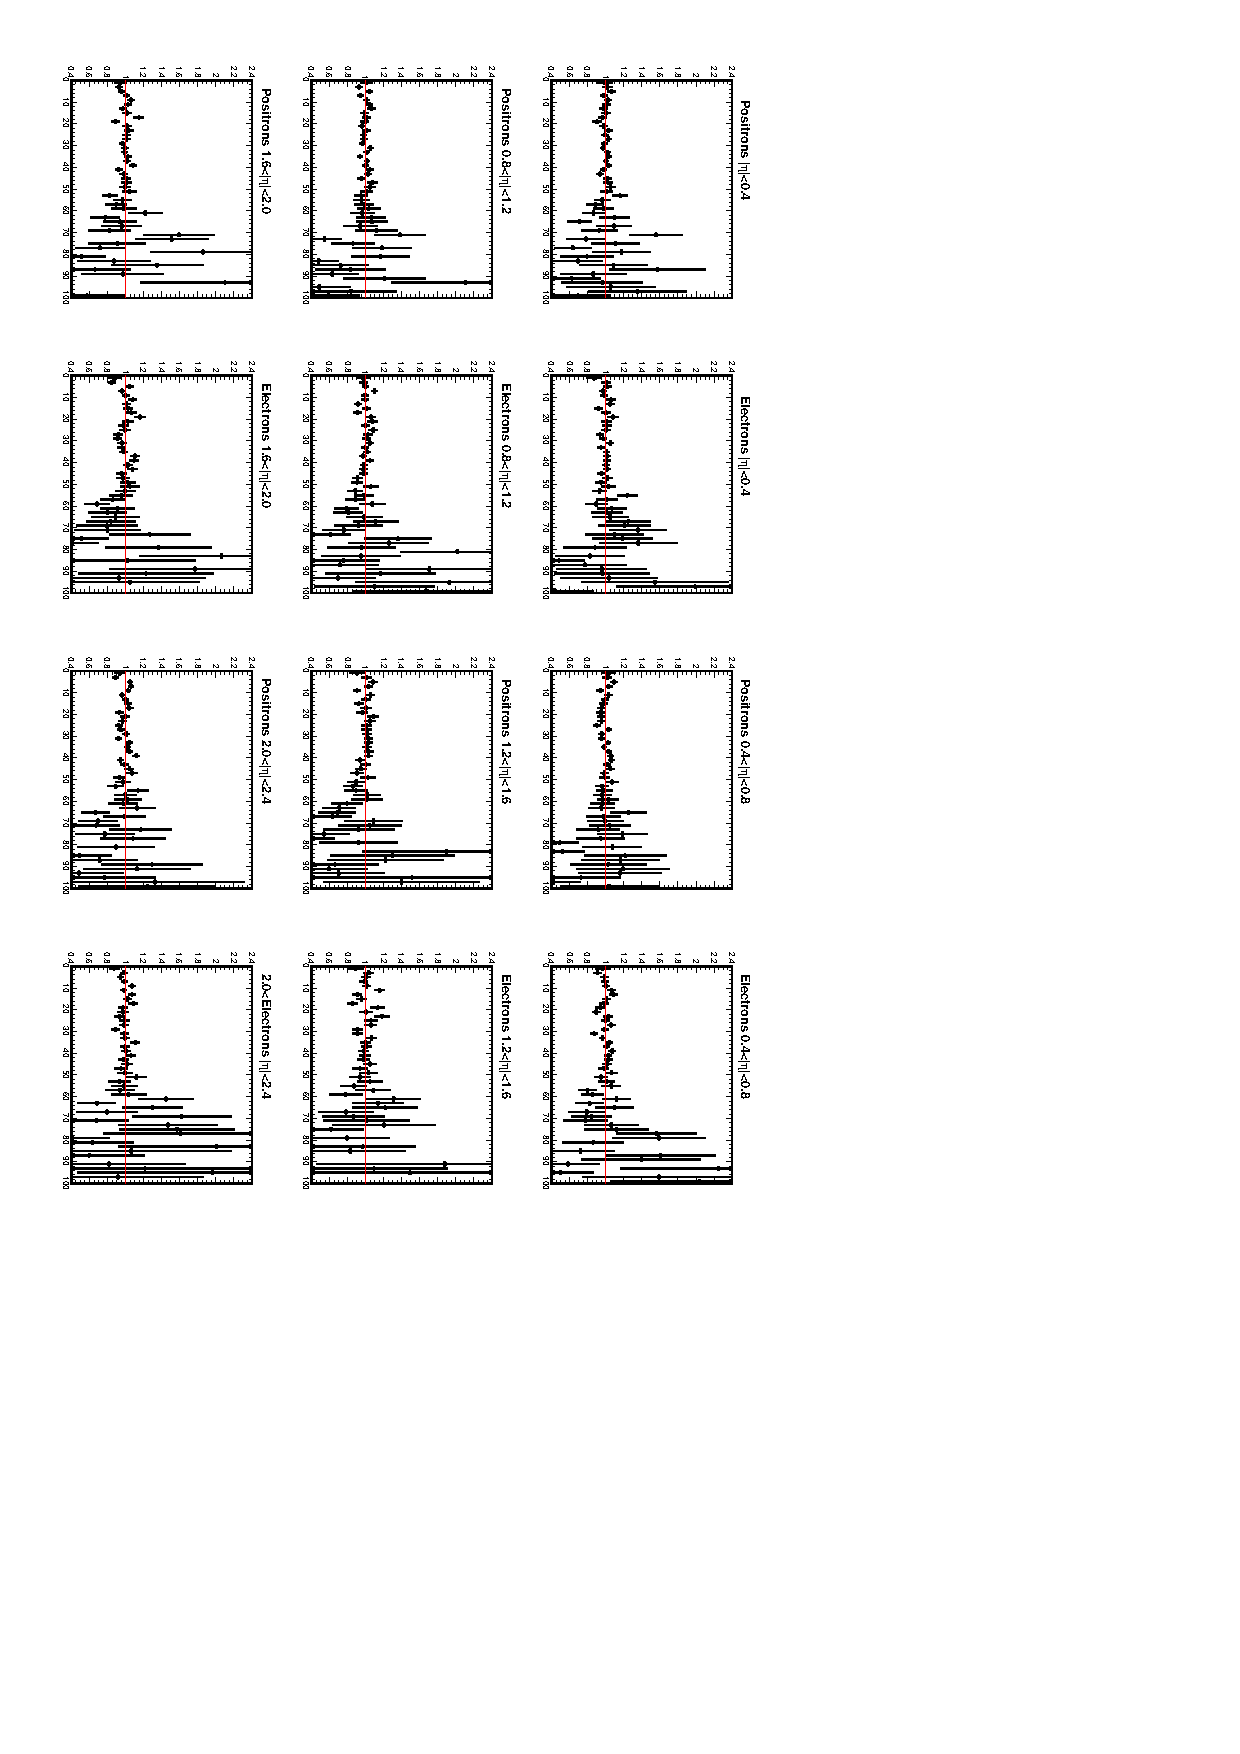
\includegraphics[trim = 80mm 100mm 0mm 0mm, clip, angle=90, width=0.95\textwidth]{Dec22_fitratio}
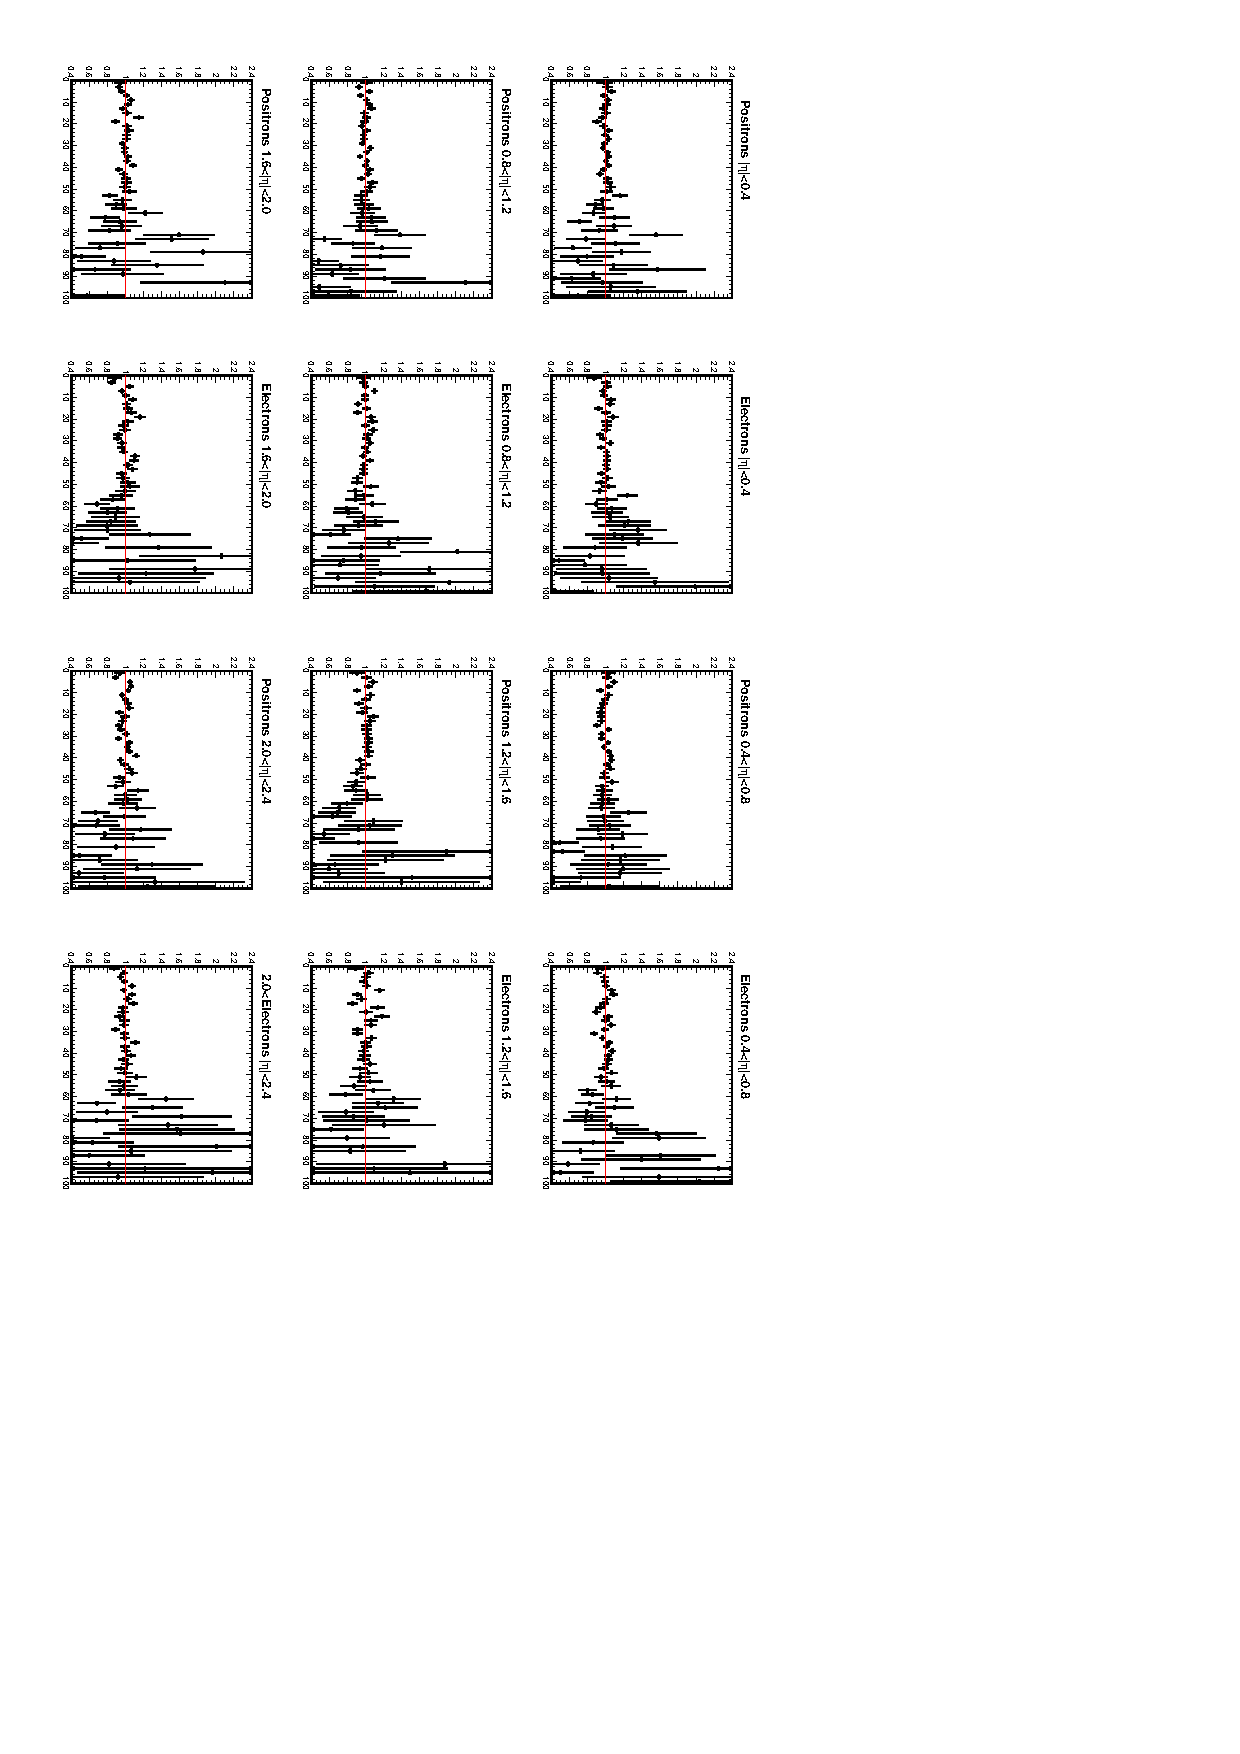
\includegraphics[trim = 80mm 0mm 0mm 100mm, clip, angle=90, width=0.95\textwidth]{Dec22_fitratio}
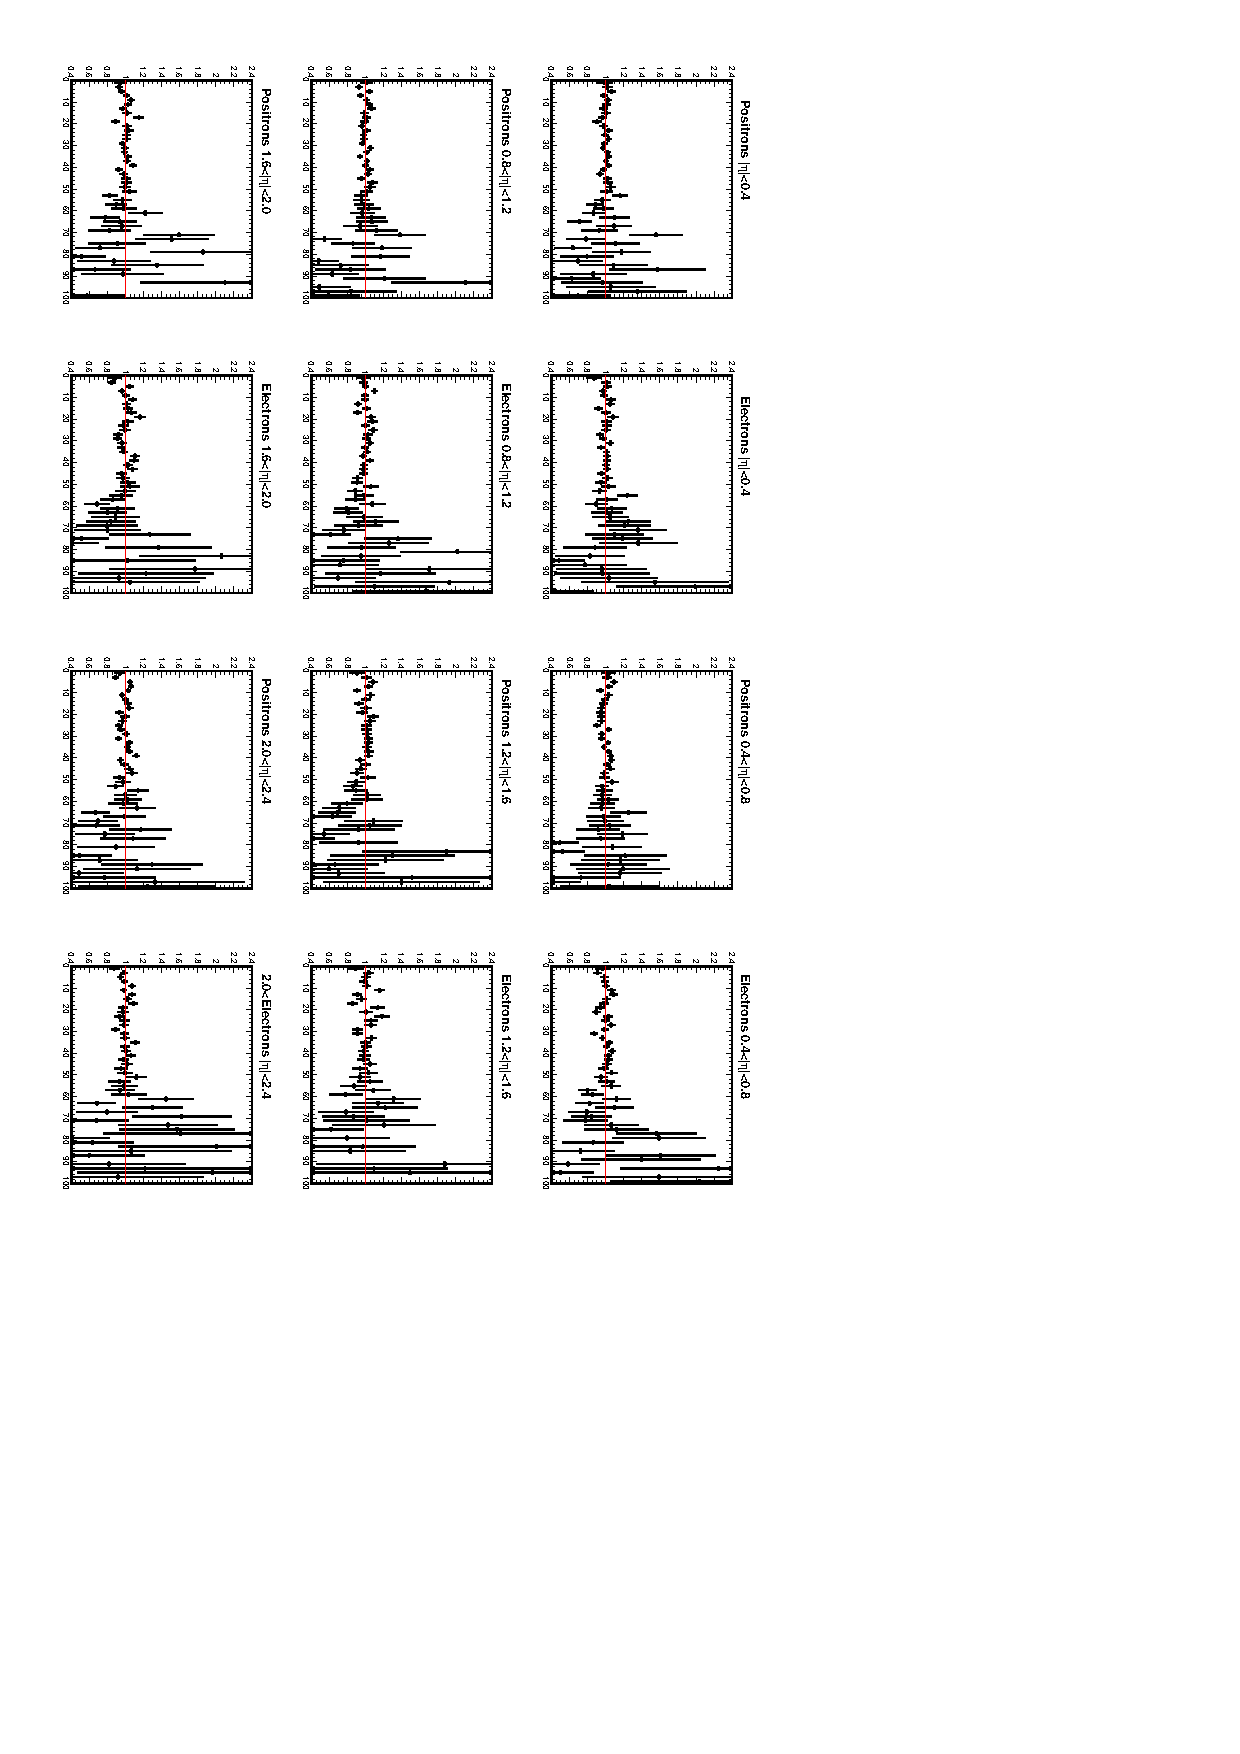
\includegraphics[trim = 40mm 100mm 40mm 0mm, clip, angle=90, width=0.95\textwidth]{Dec22_fitratio}
     \caption{\label{fig:fit1ratio}Ratio between fit and data for each eta/charge bin.}
  \end{center}
\end{figure}

\begin{figure}
  \begin{center}
% bottom right top left
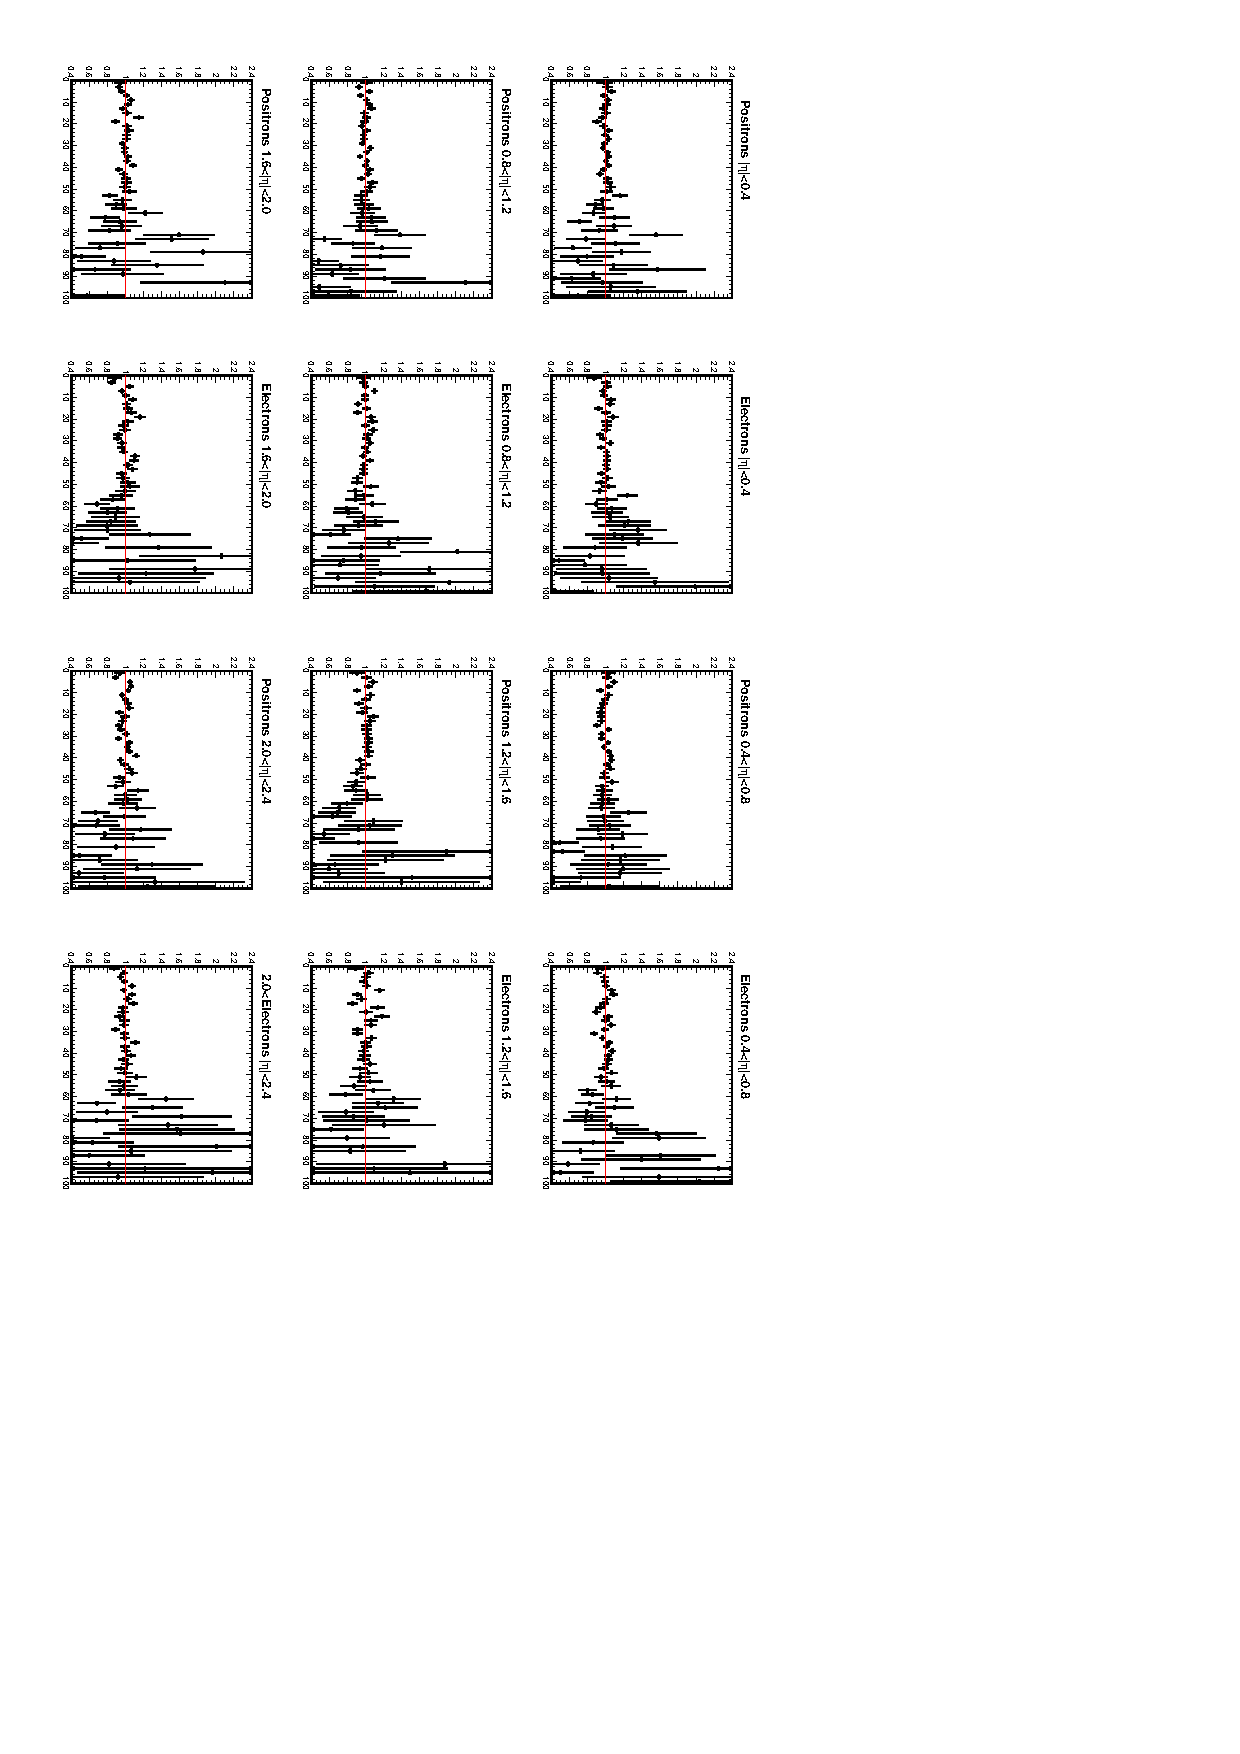
\includegraphics[trim = 40mm 0mm 40mm 100mm, clip, angle=90, width=0.95\textwidth]{Dec22_fitratio}
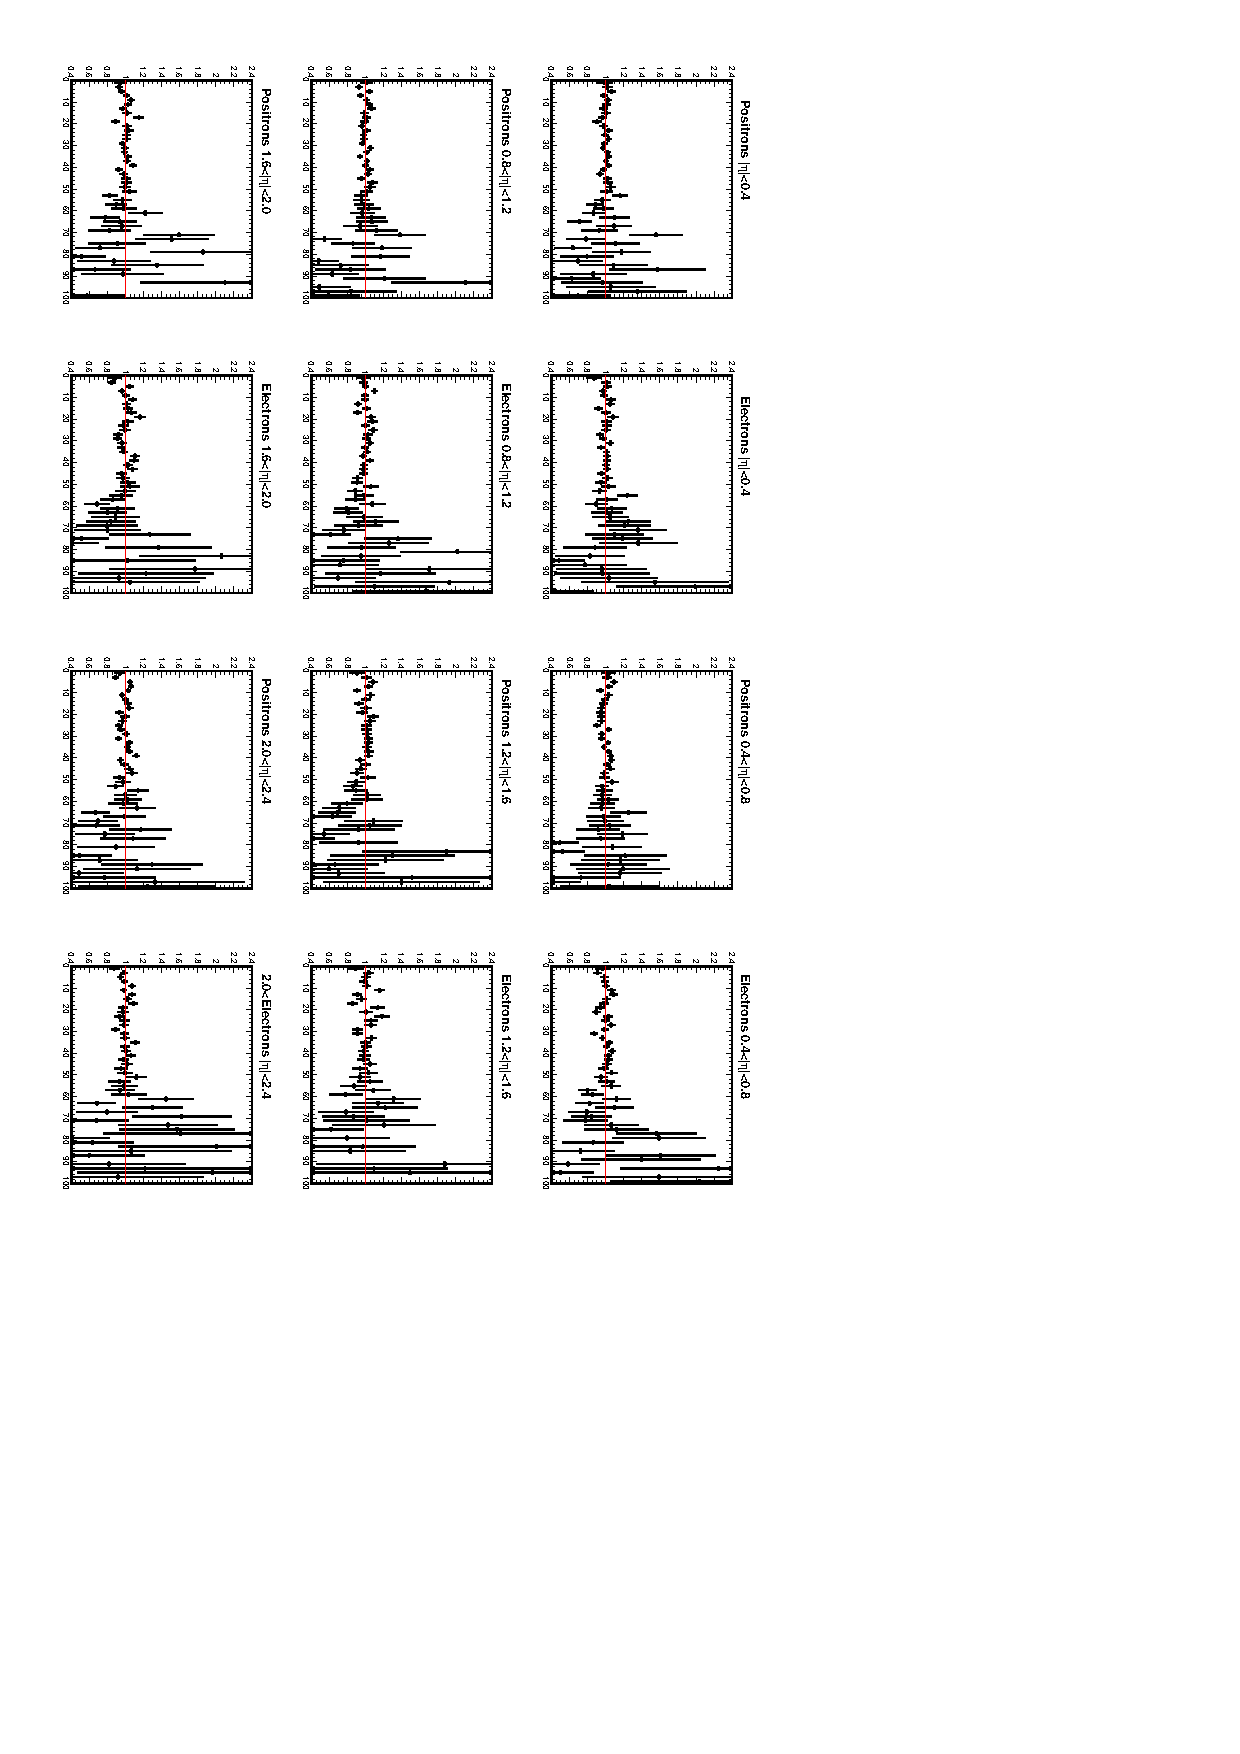
\includegraphics[trim = 0mm 100mm 80mm 0mm, clip, angle=90, width=0.95\textwidth]{Dec22_fitratio}
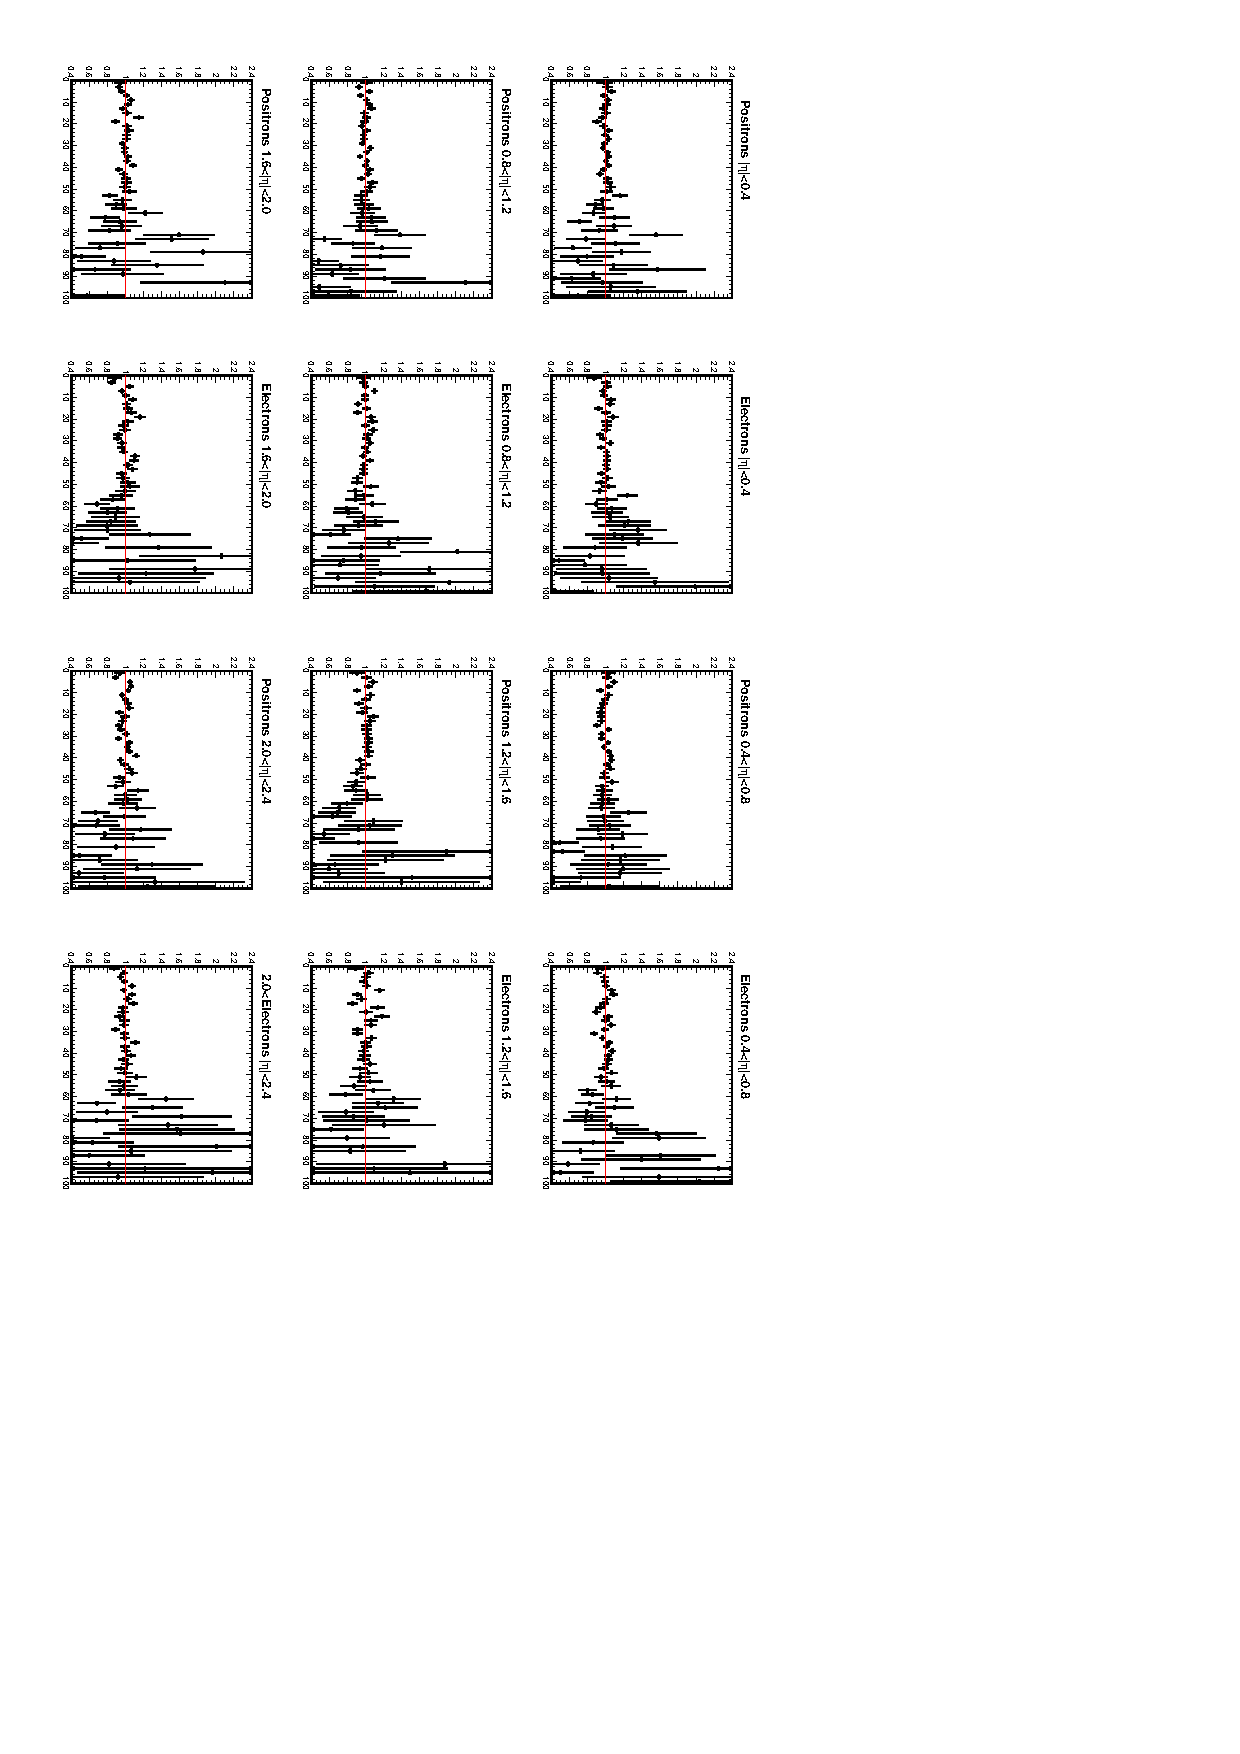
\includegraphics[trim = 0mm 0mm 80mm 100mm, clip, angle=90, width=0.95\textwidth]{Dec22_fitratio}
     \caption{\label{fig:fit2ratio}Ratio between fit and data for each eta/charge bin.}
  \end{center}
\end{figure}

\clearpage

\section{\unit{840}{\invpb}}

\begin{figure}
  \begin{center}
    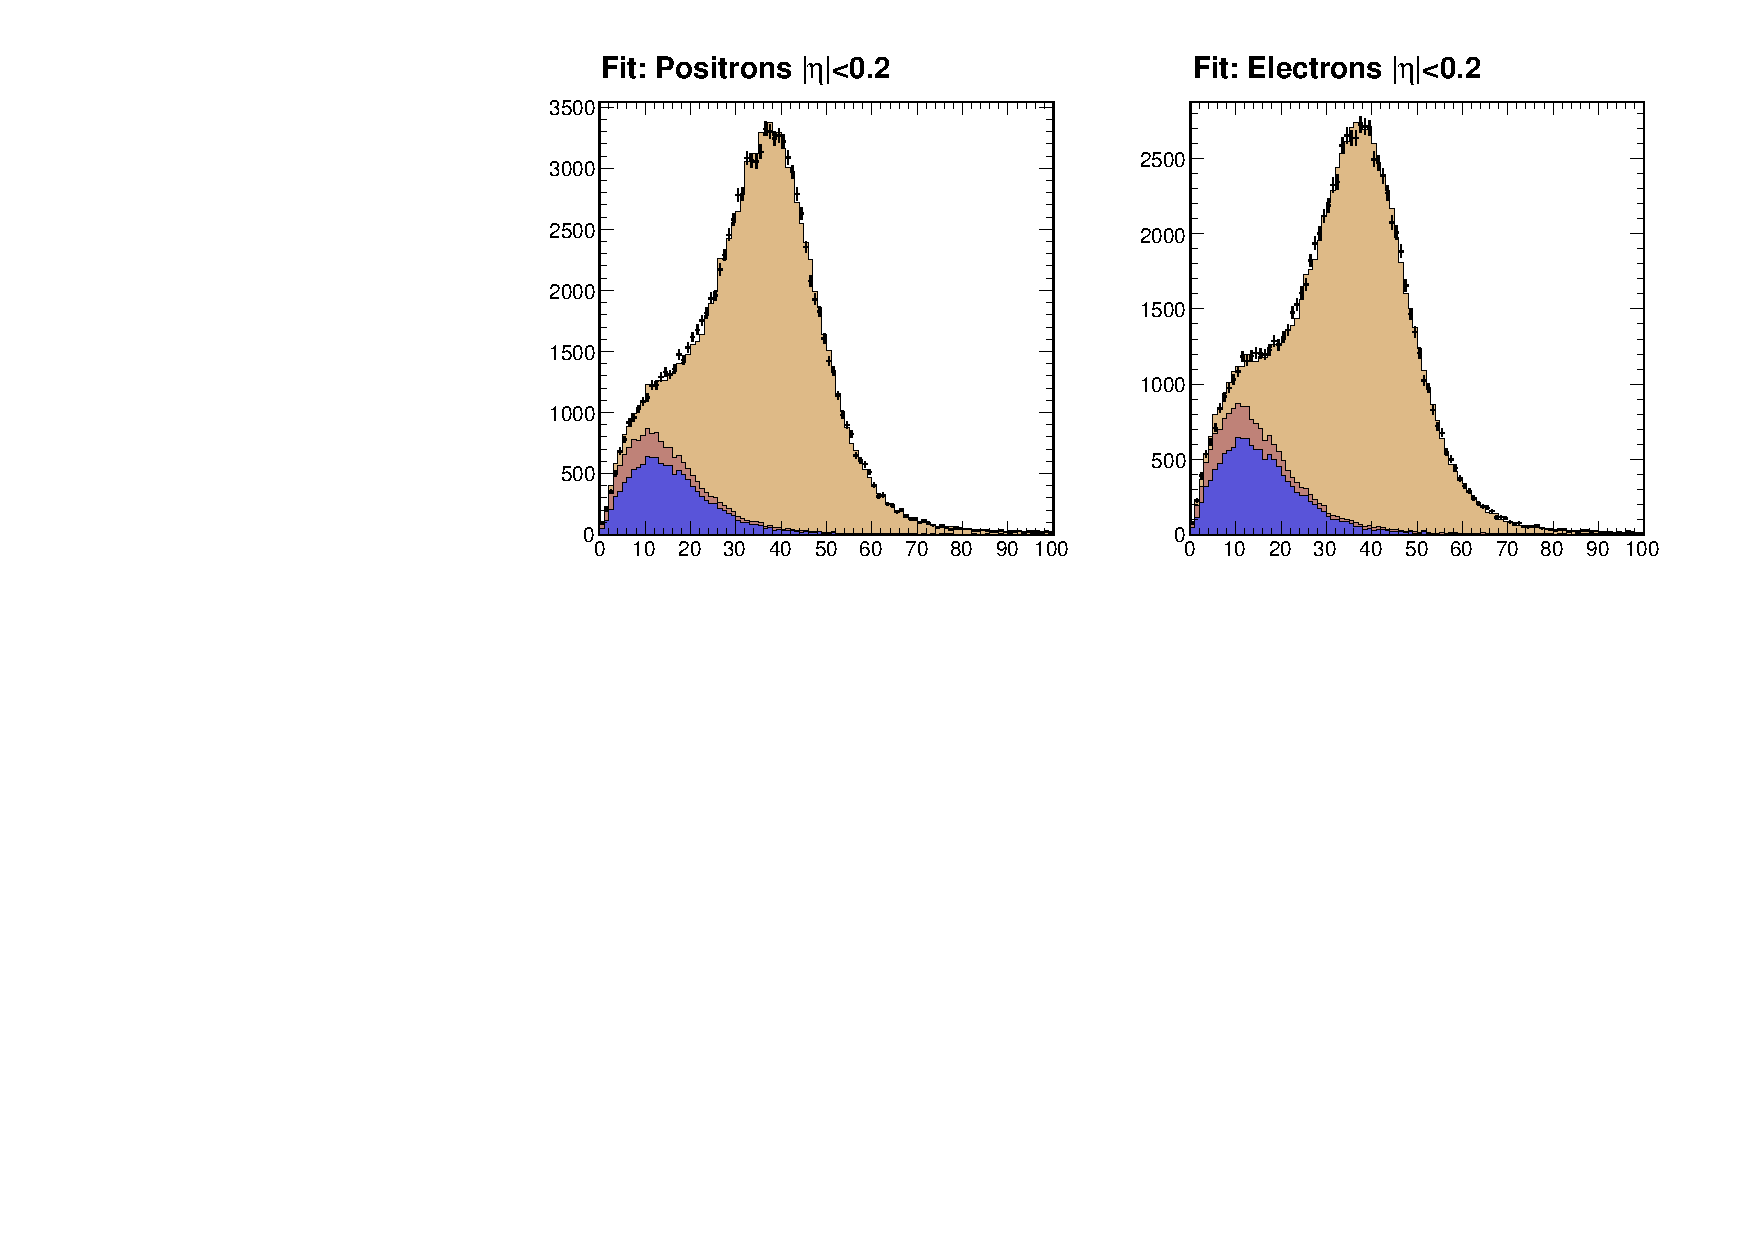
\includegraphics[width=0.95\textwidth]{data_0.pdf} \\
    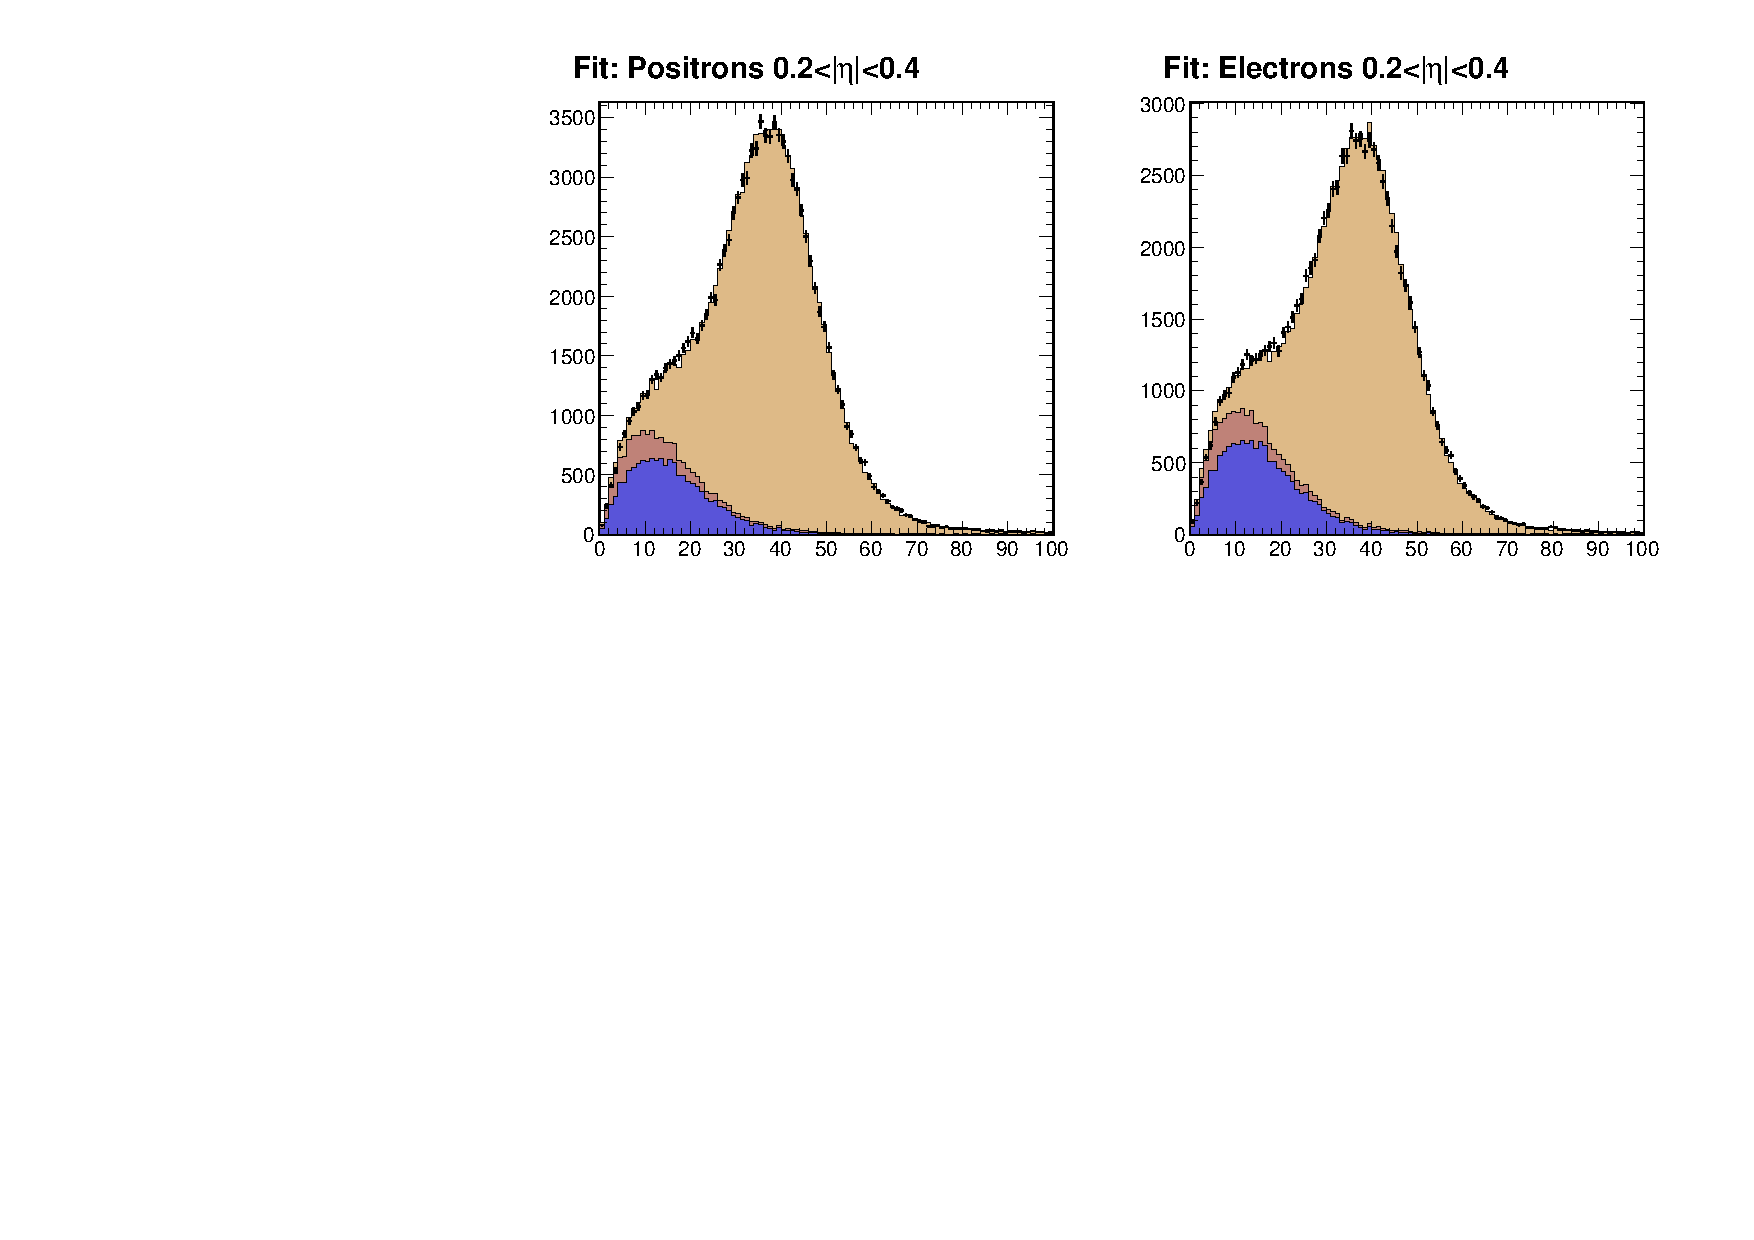
\includegraphics[width=0.95\textwidth]{data_1.pdf} \\
    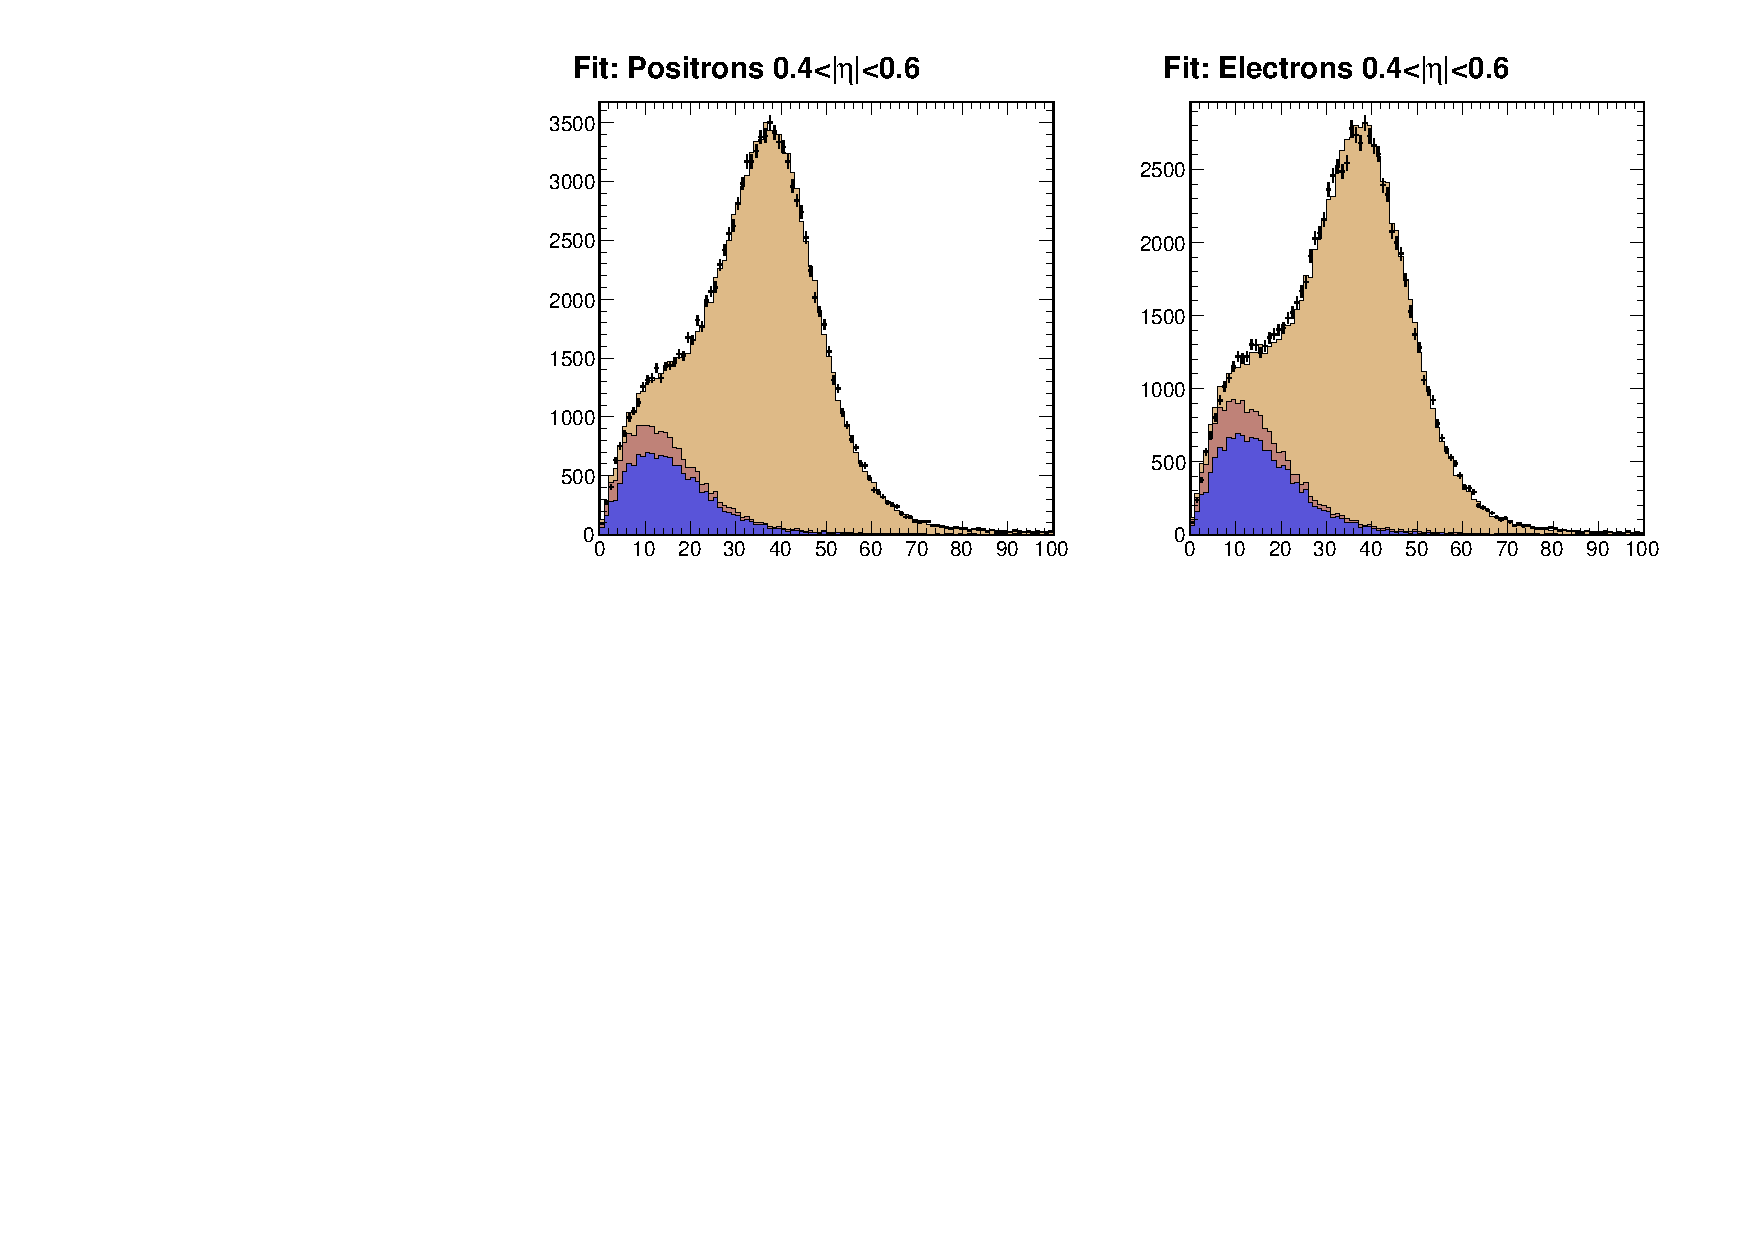
\includegraphics[width=0.95\textwidth]{data_2.pdf}
 \caption{  \label{fig:data1} The fit to \MET\ for eta bins 1,2 and 3.}
  \end{center}
\end{figure}

\begin{figure}
  \begin{center}
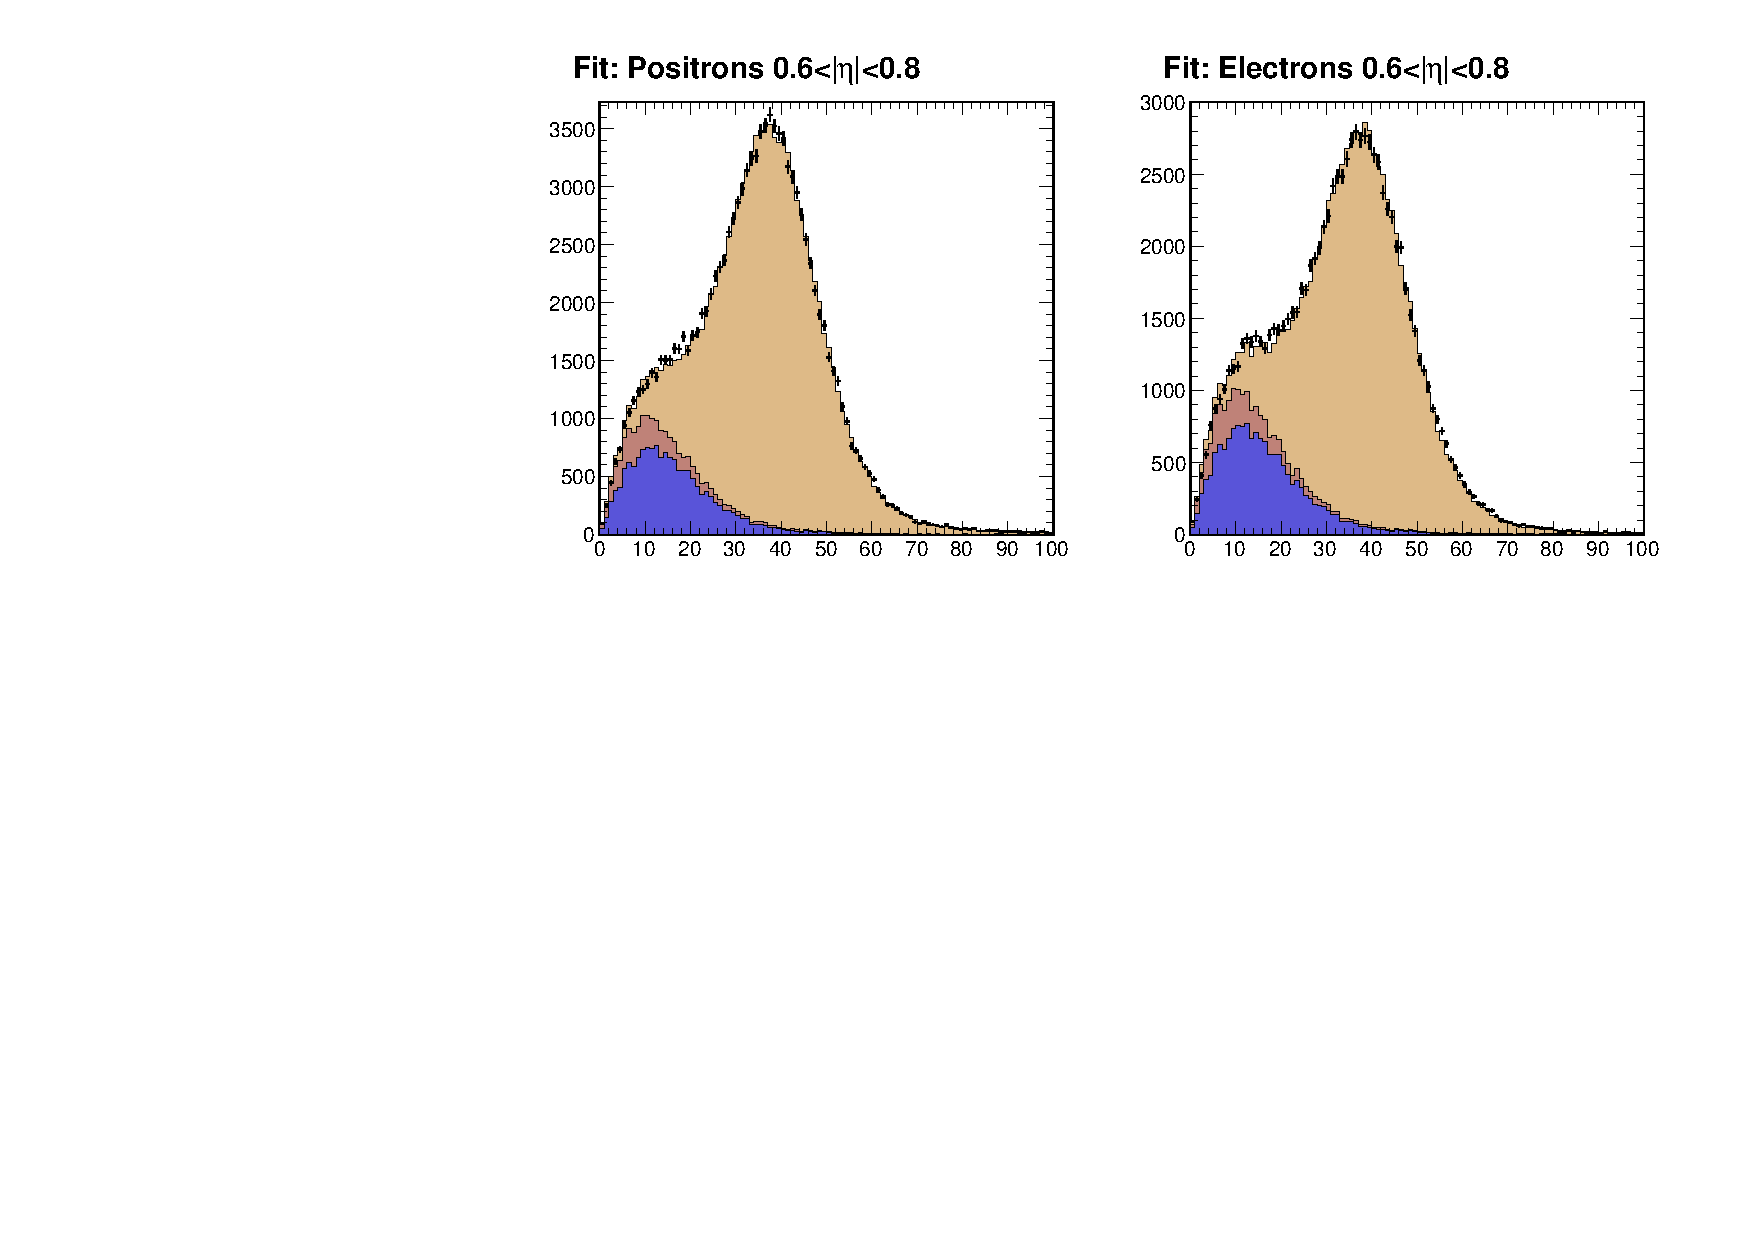
\includegraphics[width=0.95\textwidth]{data_3.pdf} \\
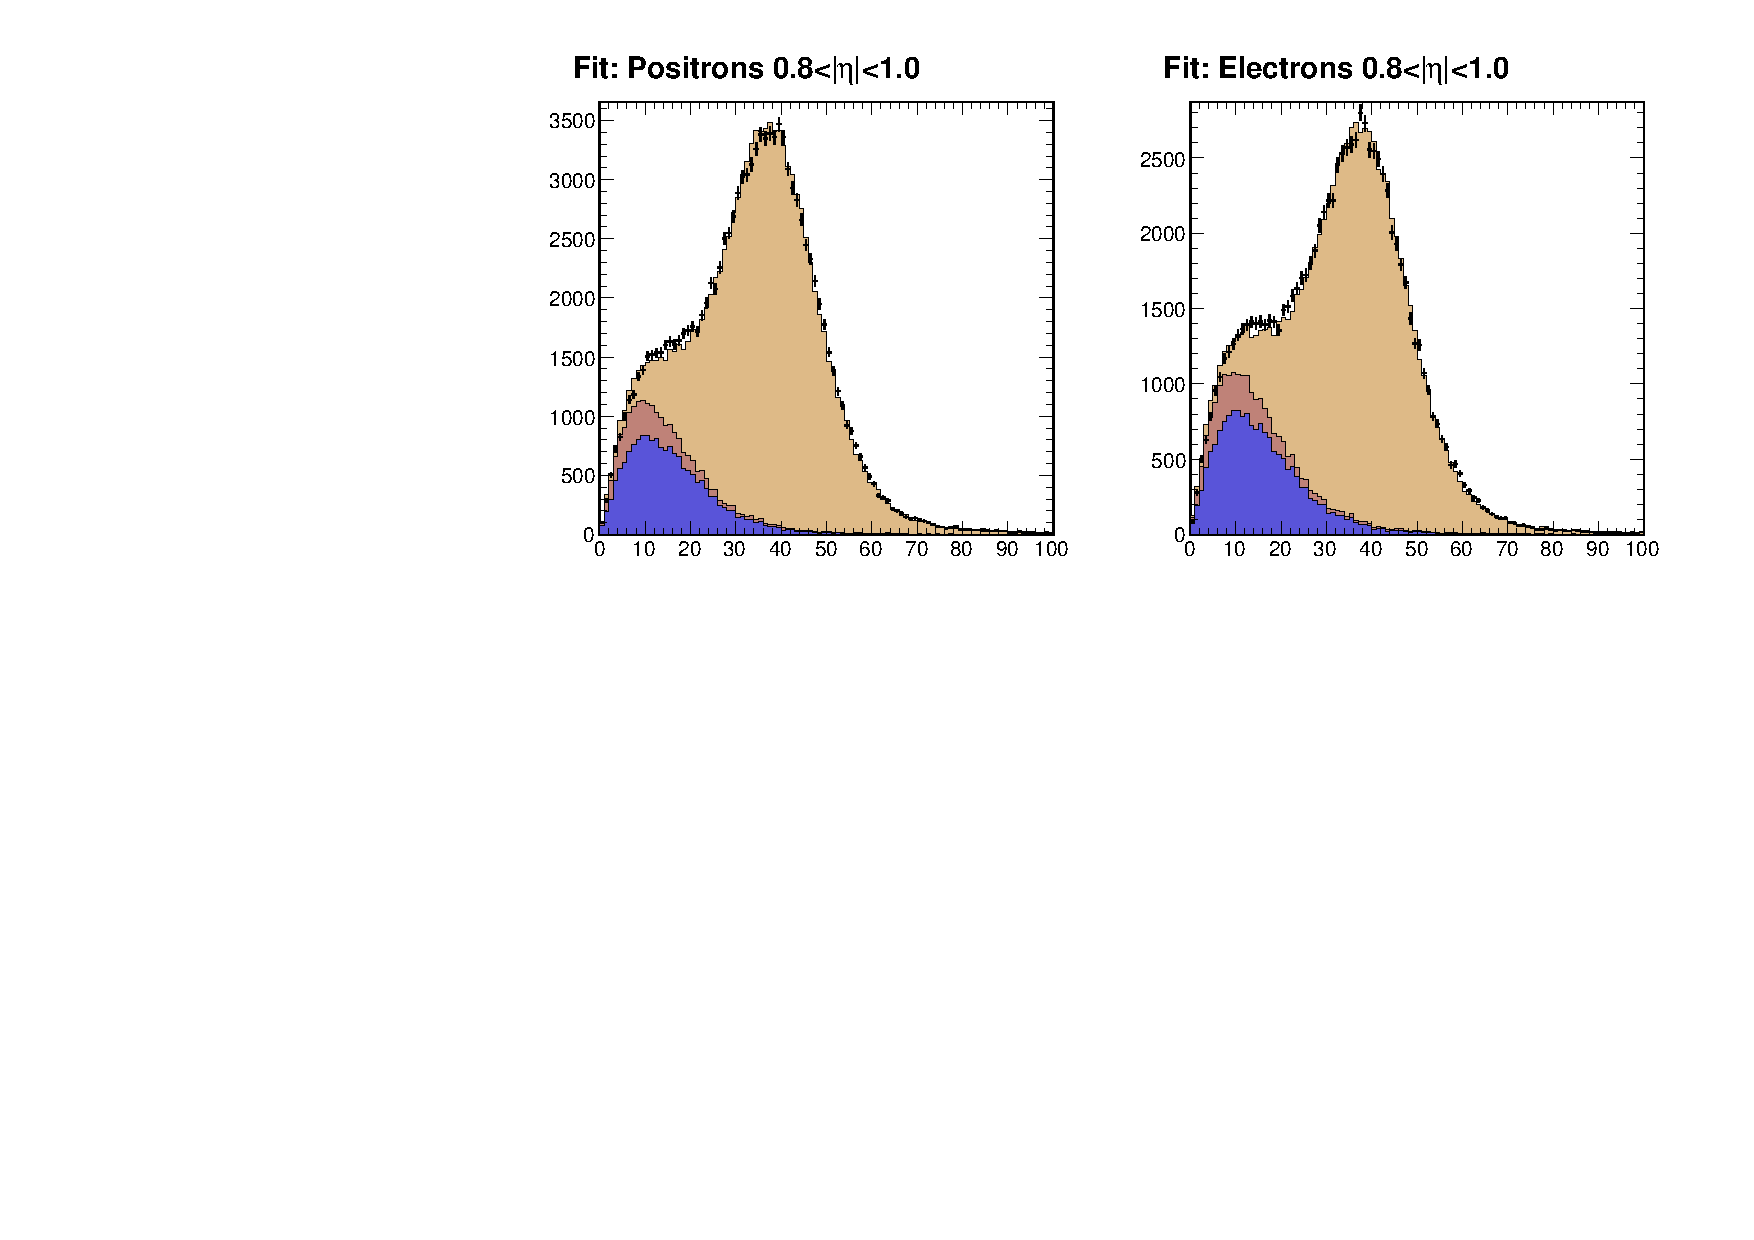
\includegraphics[width=0.95\textwidth]{data_4.pdf} \\
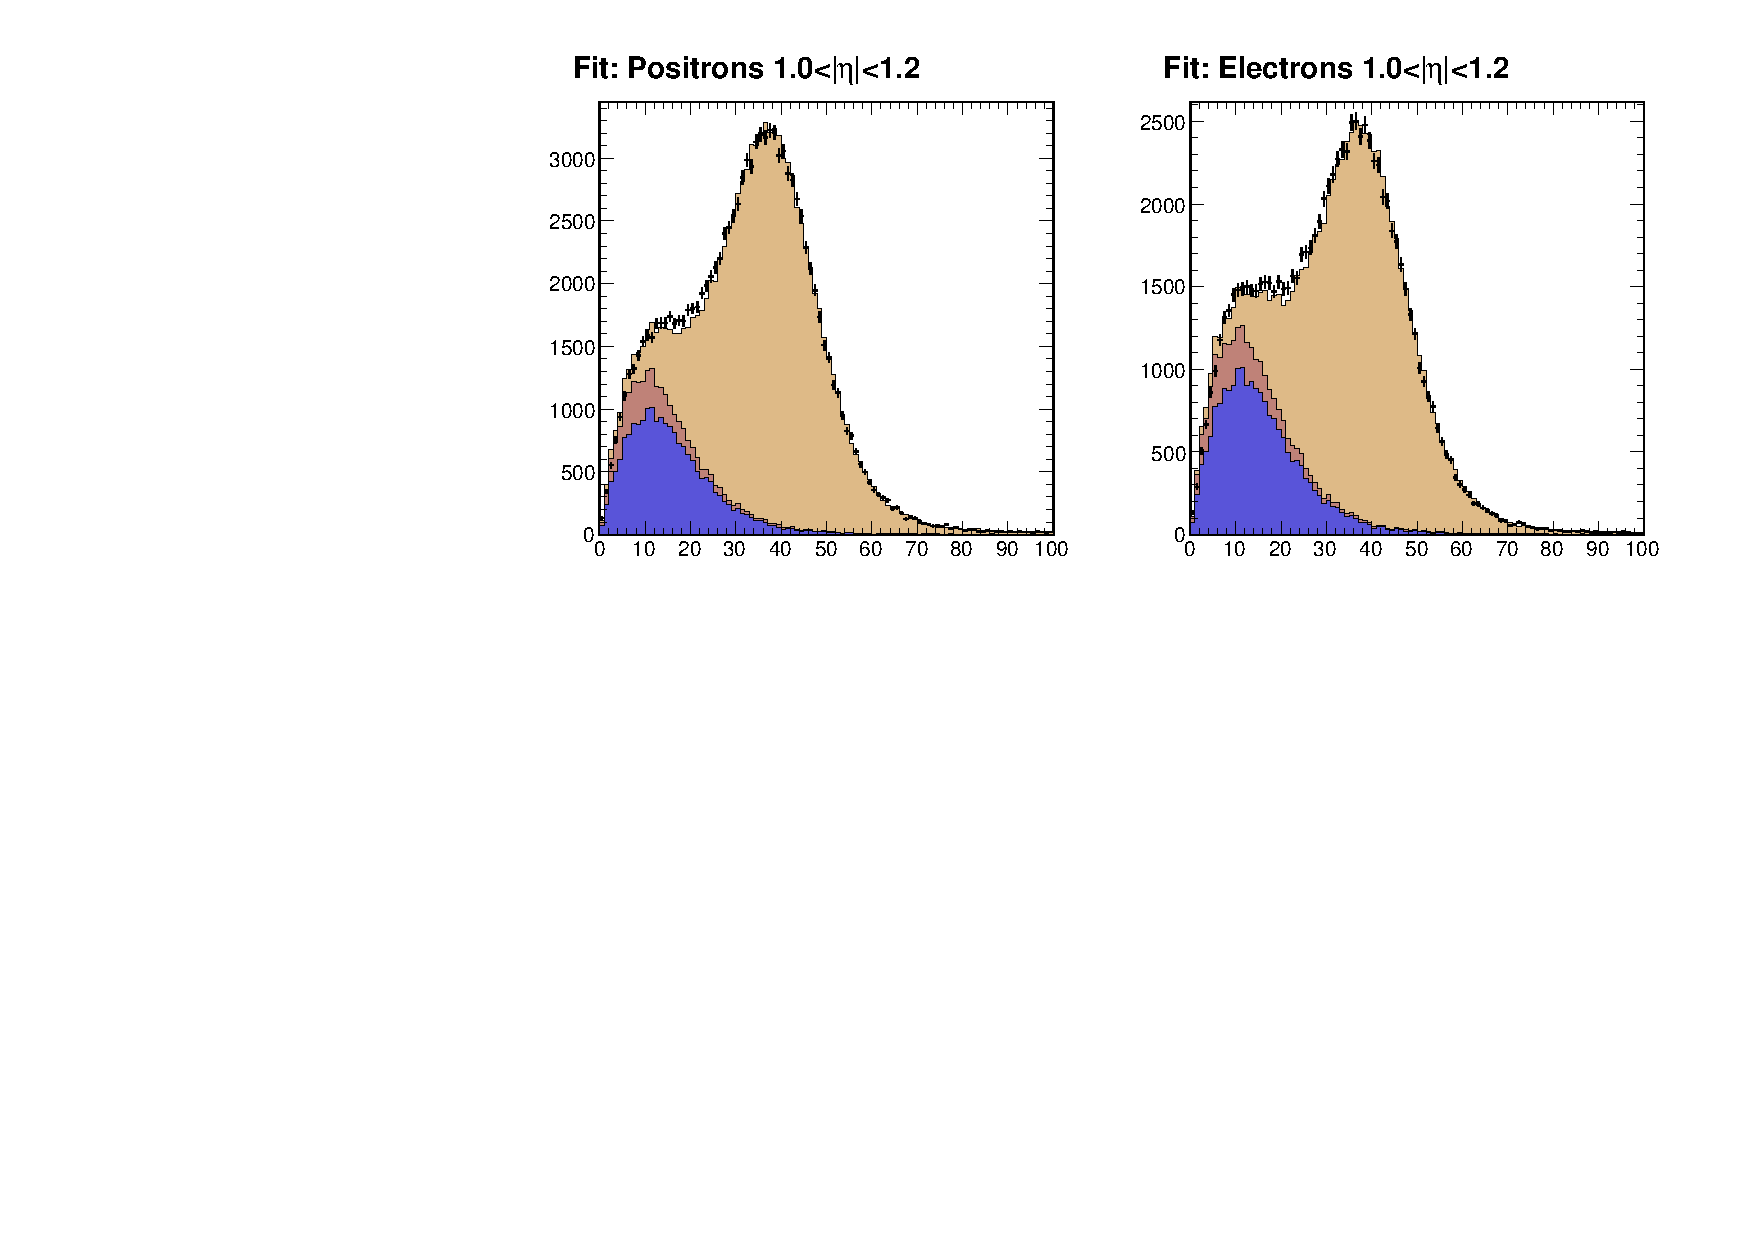
\includegraphics[width=0.95\textwidth]{data_5.pdf}
 \caption{  \label{fig:data2} The fit to \MET\ for eta bins 4,5 and 6.}
  \end{center}
\end{figure}

\begin{figure}
  \begin{center}
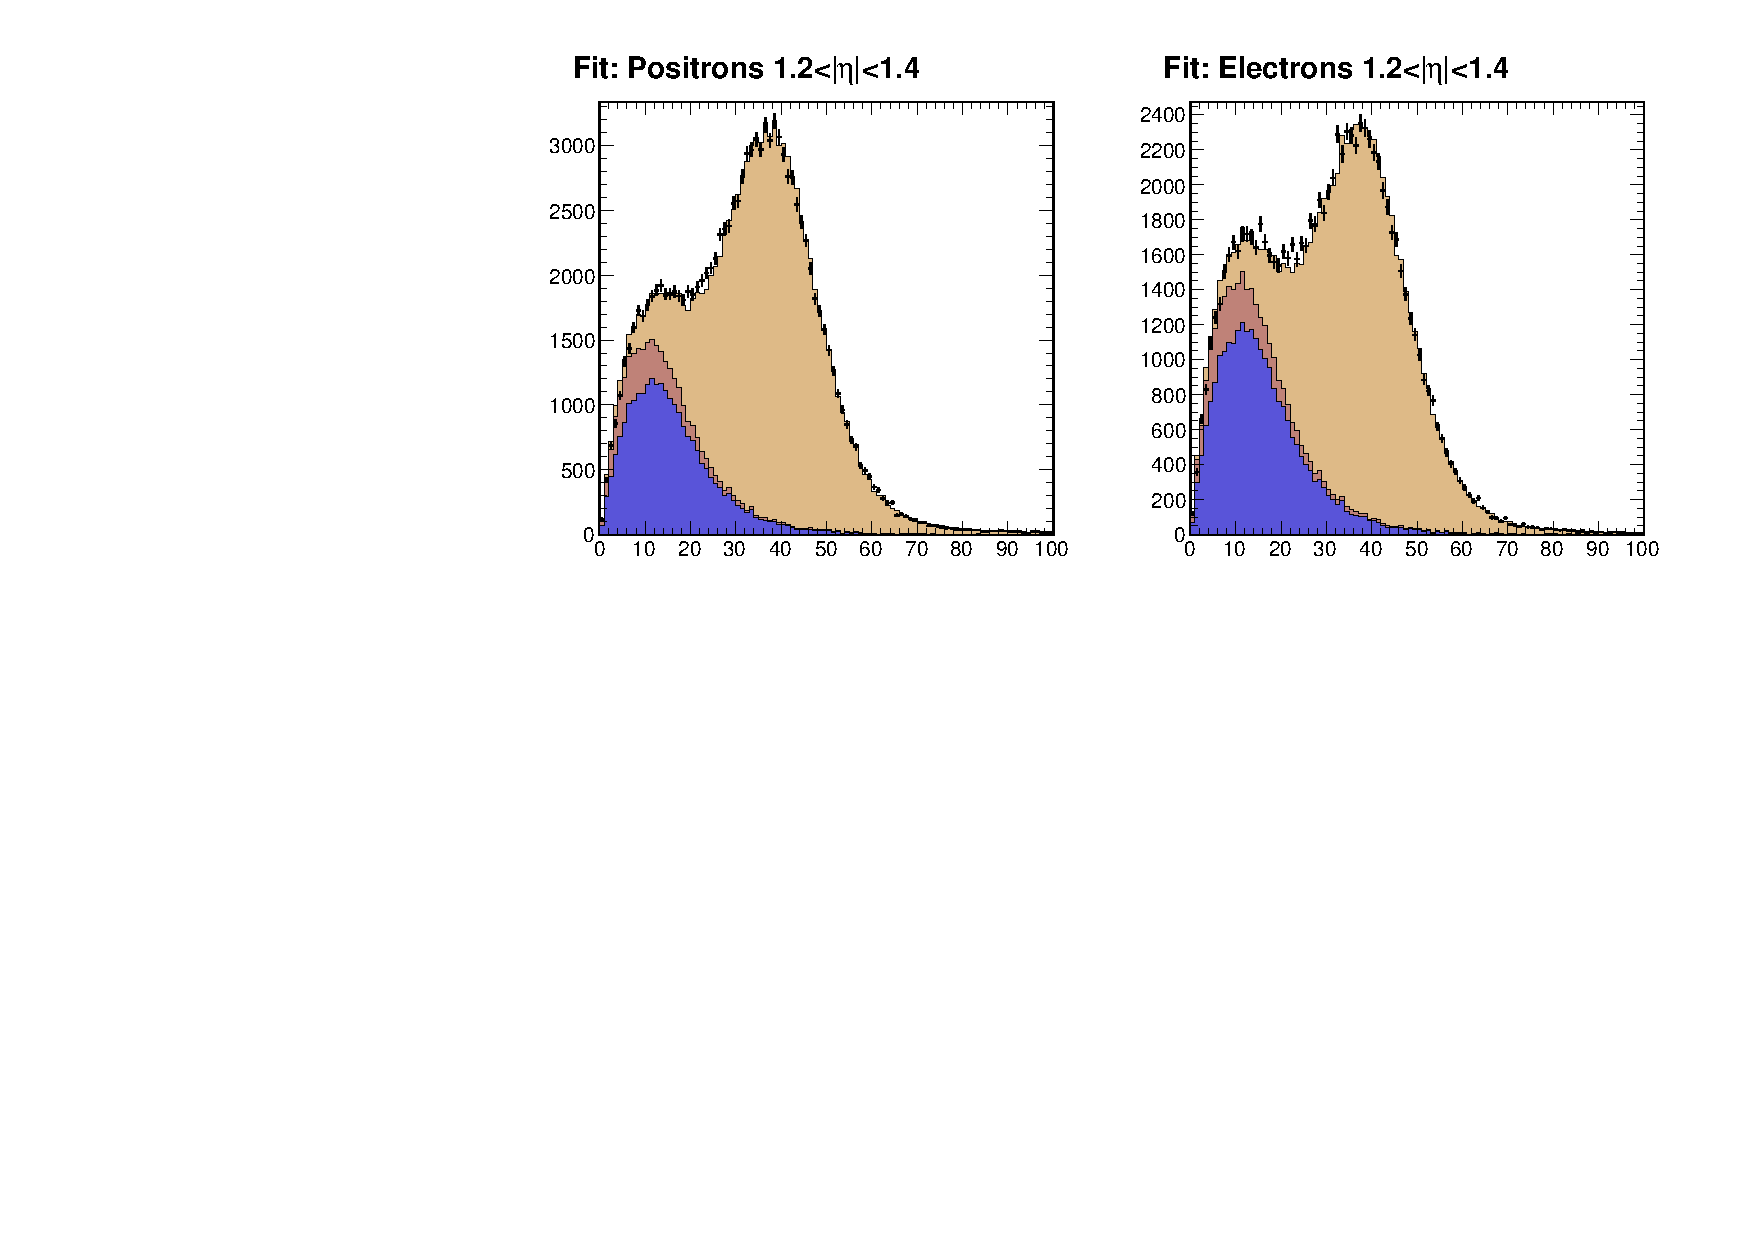
\includegraphics[width=0.95\textwidth]{data_6.pdf} \\
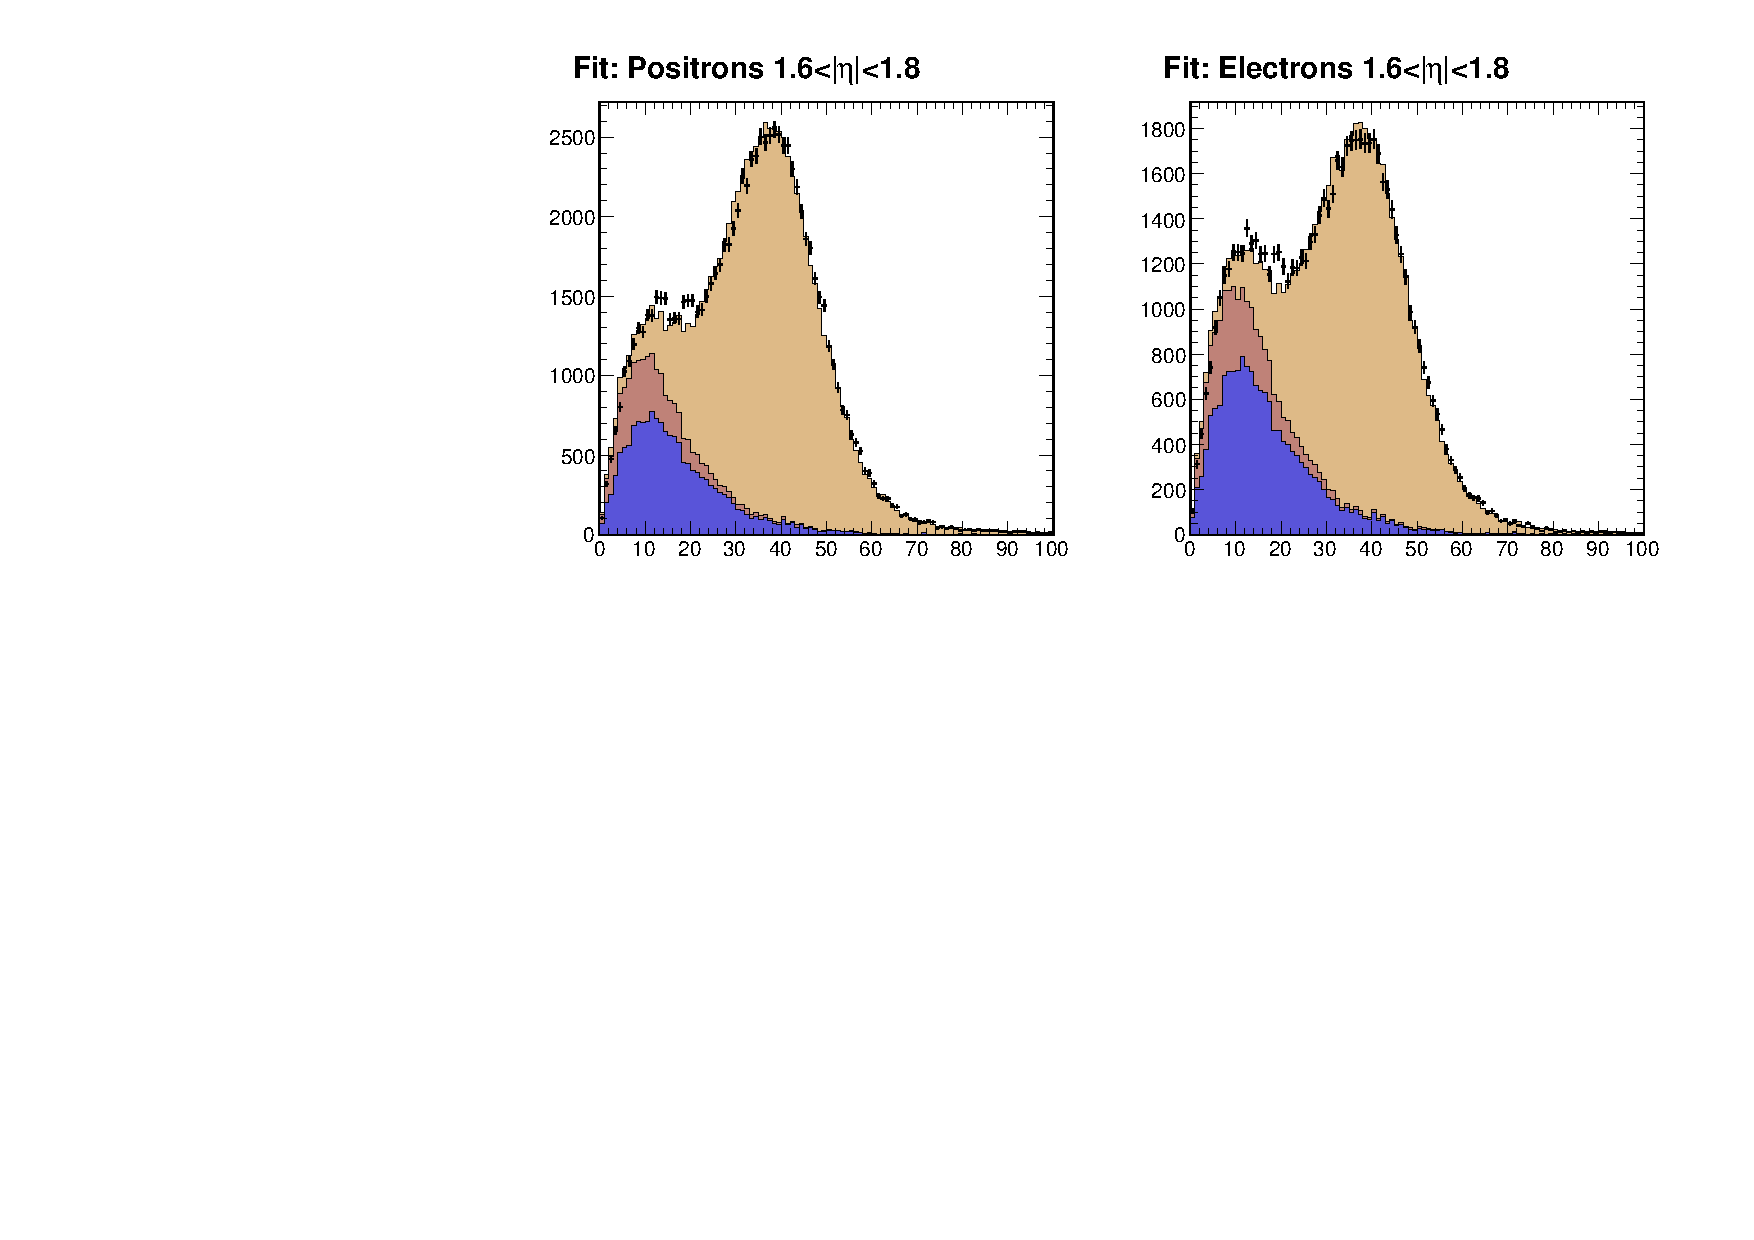
\includegraphics[width=0.95\textwidth]{data_7.pdf} \\
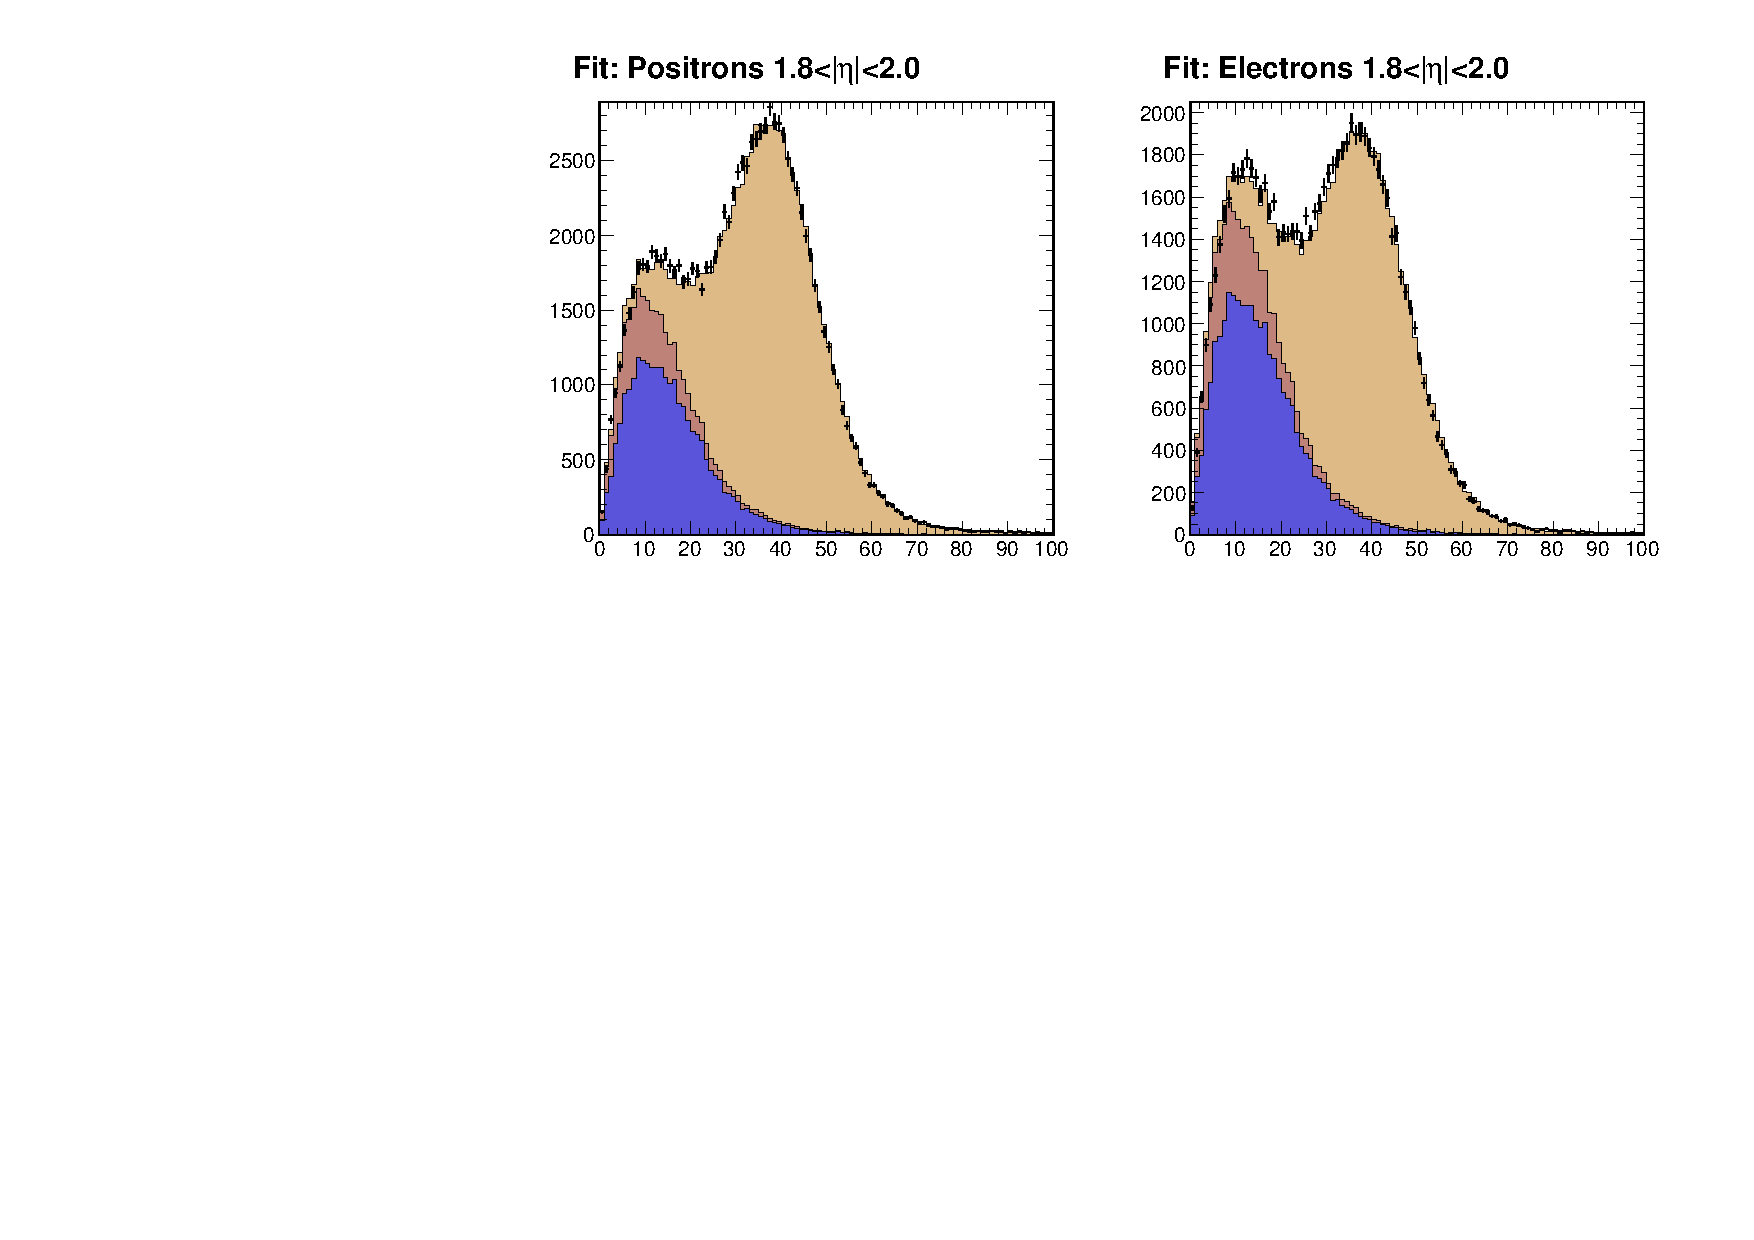
\includegraphics[width=0.95\textwidth]{data_8.pdf}
 \caption{  \label{fig:data3} The fit to \MET\ for eta bins 7,8 and 9.}
  \end{center}
\end{figure}

\begin{figure}
  \begin{center}
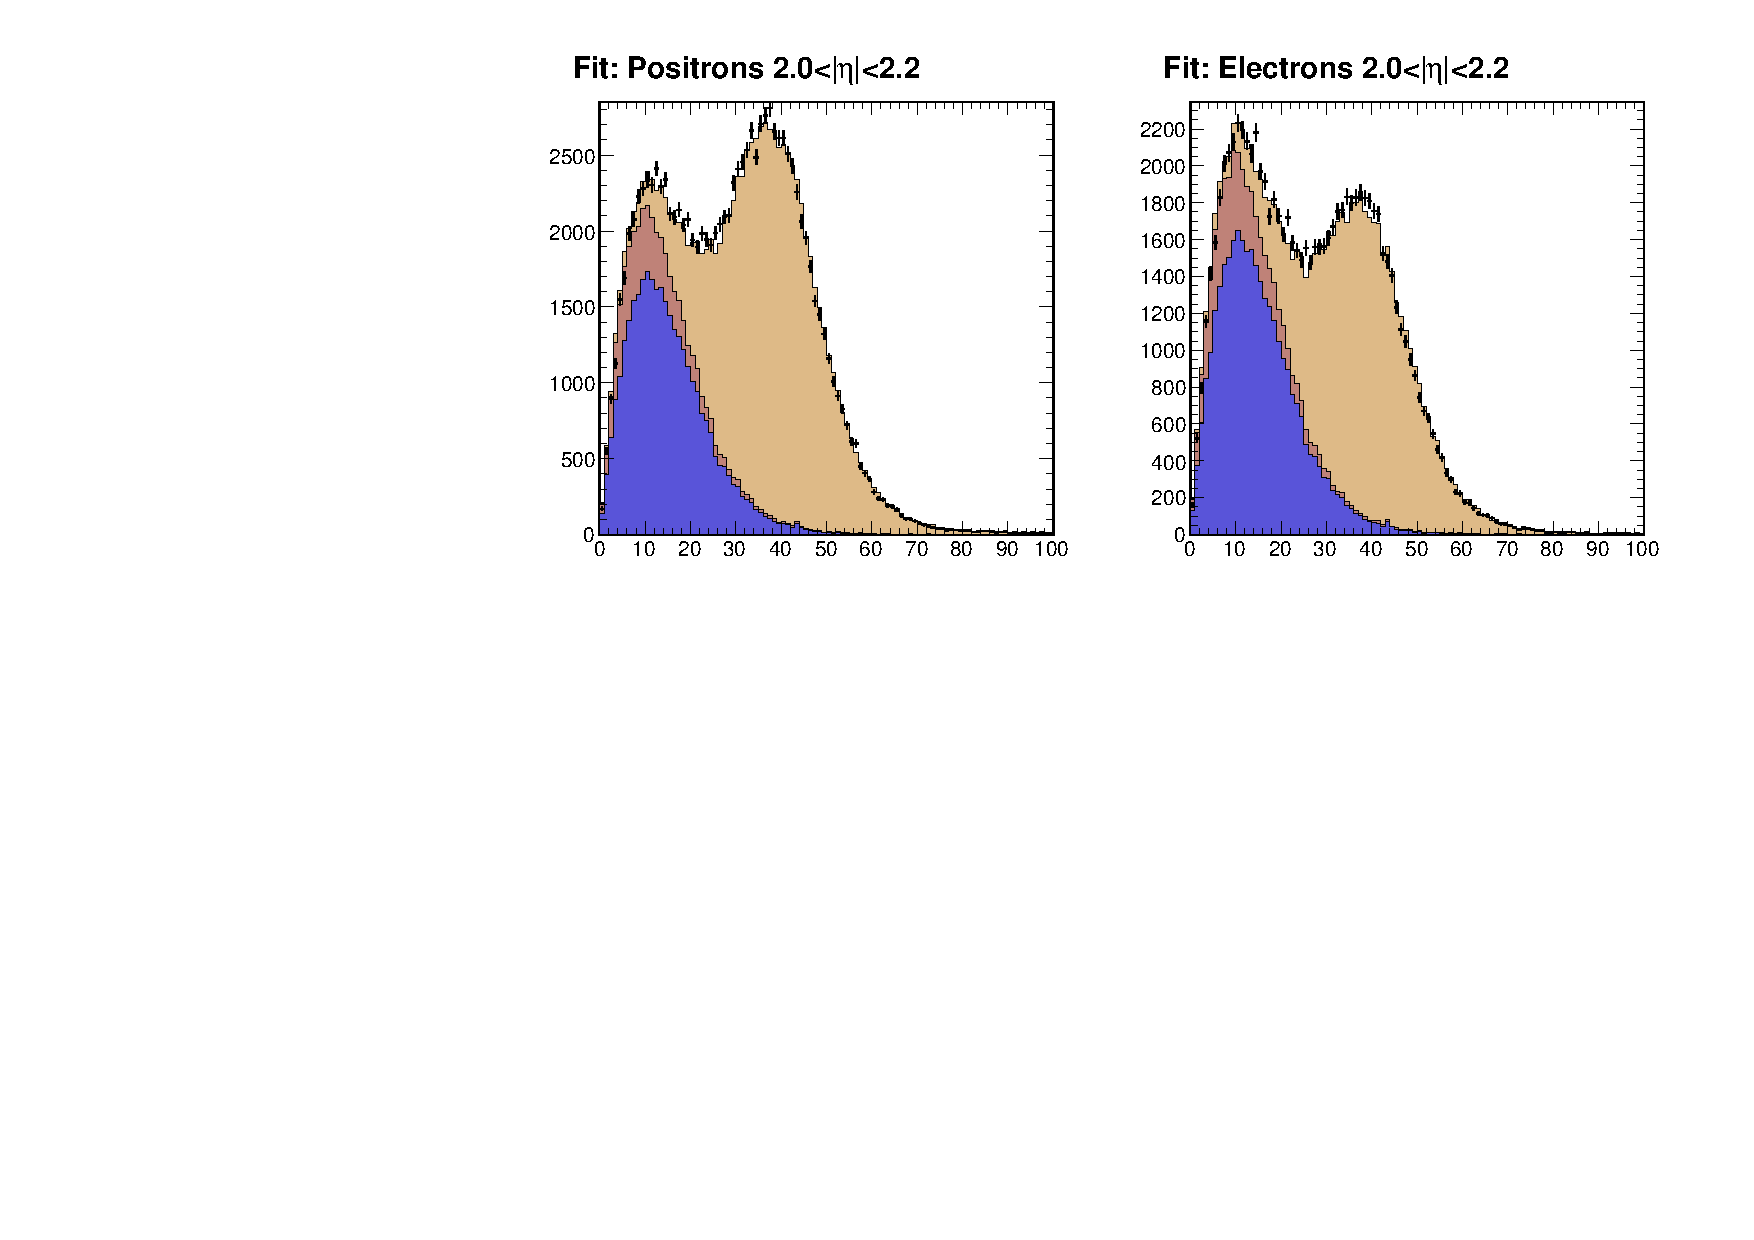
\includegraphics[width=0.95\textwidth]{data_9.pdf} \\
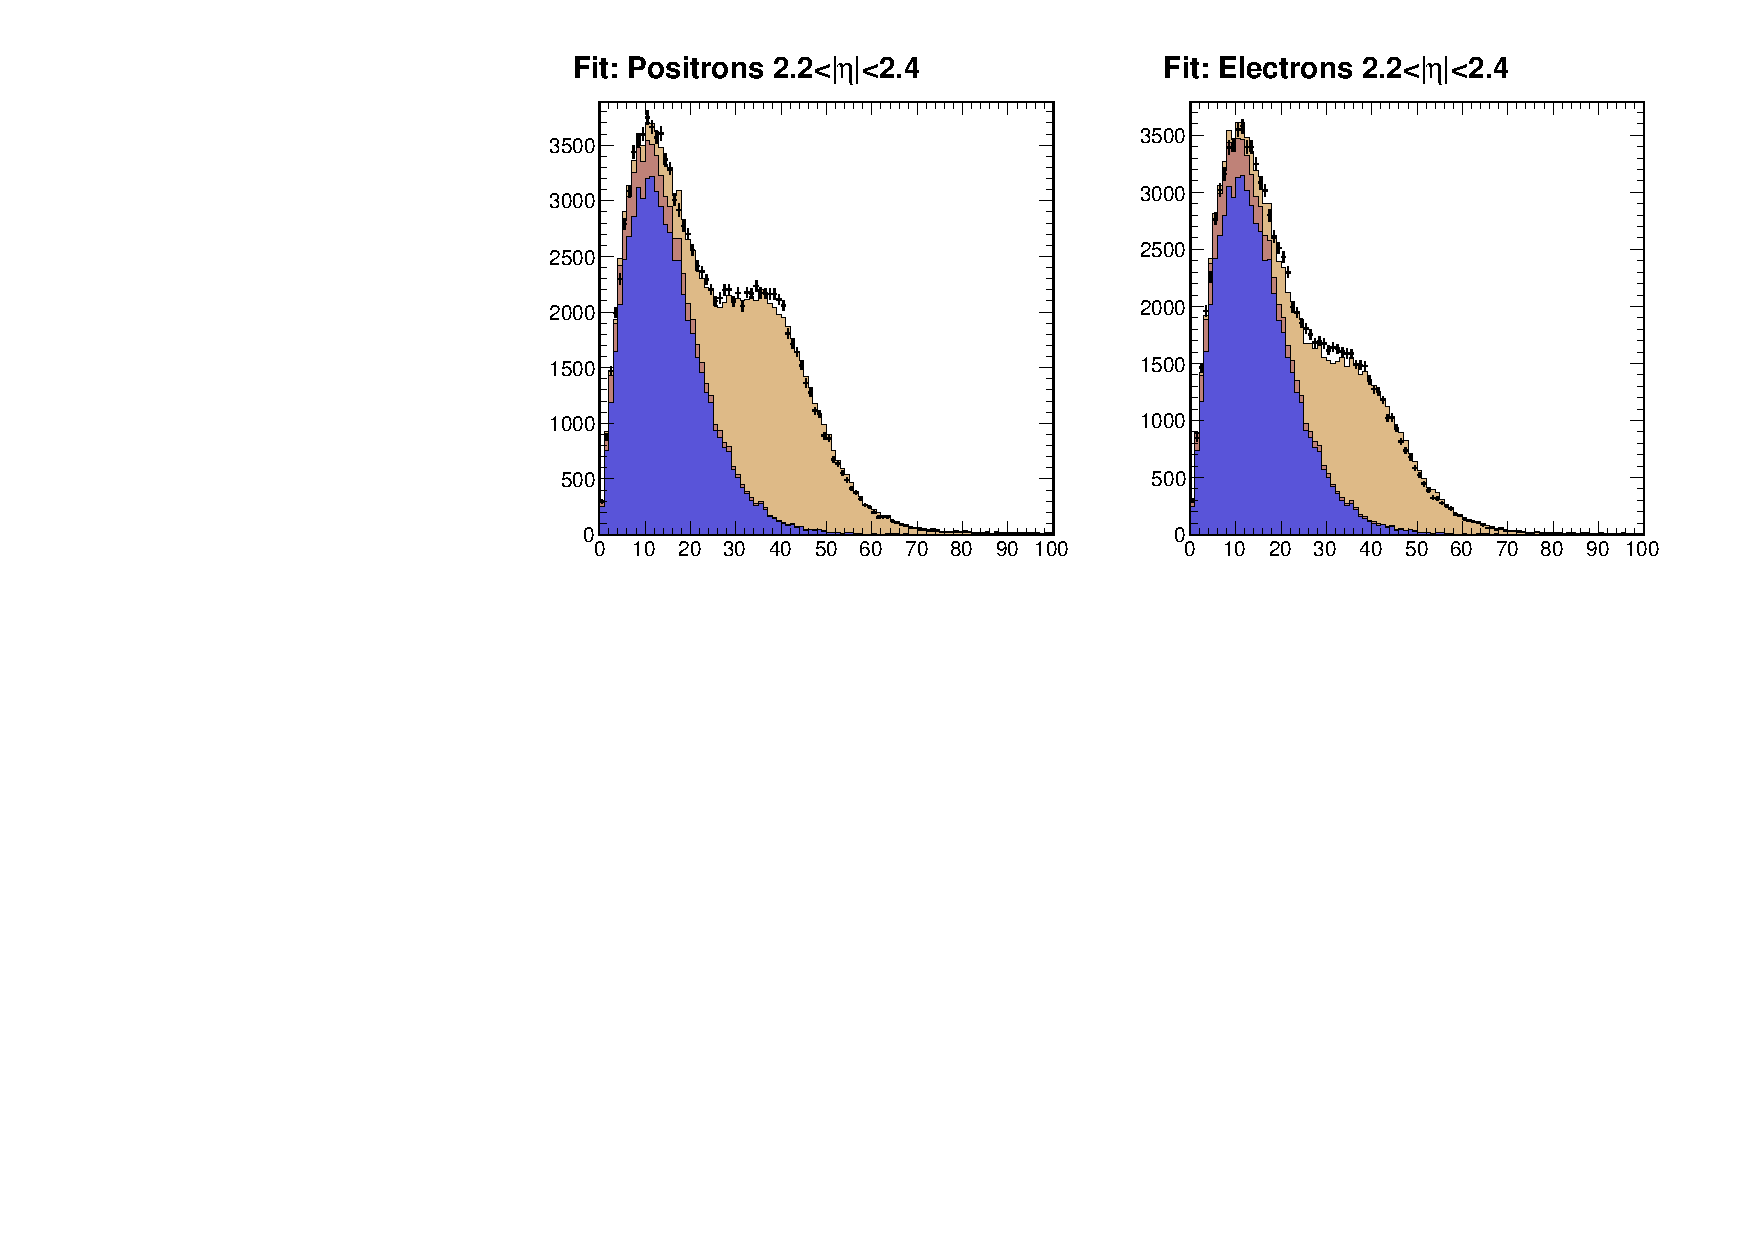
\includegraphics[width=0.95\textwidth]{data_10.pdf}
  \caption{  \label{fig:data4} The fit to \MET\ for eta bins 10 and 11.}
   \end{center}
\end{figure}

